%
% Copyright 2018 Joel Feldman, Andrew Rechnitzer and Elyse Yeager.
% This work is licensed under a Creative Commons Attribution-NonCommercial-ShareAlike 4.0 International License.
% https://creativecommons.org/licenses/by-nc-sa/4.0/
%
\questionheader{ex:s3.3}

%%%%%%%%%%%%%%%%%%
\subsection*{\Conceptual}
%%%%%%%%%%%%%%%%%%

%%%%%%%%%%%%%%%%%%
\begin{Mquestion}
Select the series below that diverge by the divergence test.

\hfill(A)~ $\displaystyle\sum_{n=1}^\infty \frac{1}{n}$ \hfill
\hfill(B)~ $\displaystyle\sum_{n=1}^\infty \frac{n^2}{n+1}$
\hfill (C)~$\displaystyle\sum_{n=1}^\infty \sin n$
\hfill(D)~ $\displaystyle\sum_{n=1}^\infty \sin (\pi n)$\hfill~
\end{Mquestion}
\begin{hint}
That is, which series have terms whose limit is not zero?
\end{hint}
\begin{answer}
(B), (C)
\end{answer}
\begin{solution}
\begin{enumerate}[(A)]
\item $\displaystyle\lim_{n \to \infty}\frac{1}{n}=0$, so the divergence test is inconclusive. It's true that this series diverges, but we can't show it using the divergence test.
\item $\displaystyle\lim_{n \to \infty}\frac{n^2}{n+1}=\infty$, which is not zero, so the divergence test tells us this series diverges.
\item 
We'll show below that $\displaystyle\lim_{n \to \infty}\sin n$ does not exist
at all. In particular, it is not zero. Therefore, the divergence test tells us this series diverges.

Now we'll show that $\displaystyle\lim_{n \to \infty}\sin n$ does not exist.
Suppose that it does exist and takes the value $S$. We will now see that this assumption leads to a contradiction. Add together the two 
trig identities (see Appendix \eref{CLP101}{sec trig add} in the CLP-2 text) 
\begin{align*}
\sin(n+1)  &=  \sin(n)\cos(1)+\cos(n)\sin(1) \\
\sin(n-1)  &=  \sin(n)\cos(1)-\cos(n)\sin(1) 
\end{align*}
This gives 
\begin{equation*}
\sin(n+1) +\sin (n-1) = 2\sin(n)\cos(1)
\end{equation*}
Taking the limit $n\rightarrow\infty$ gives $2S=2S\cos(1)$. Since $\cos(1)\ne 1$,
this forces $S=0$. Now the first trig identity above gives
\begin{equation*}
\cos(n)  =  \frac{\sin(n+1)-\sin(n)\cos(1)}{\sin(1)}
\end{equation*}
Taking the limit as $n\rightarrow\infty$ of that gives
\begin{equation*}
\lim_{n\to\infty}\cos(n)  =  \frac{S-S\cos(1)}{\sin(1)}=0
\end{equation*}
But that provides the contradiction. Because $\sin^2(n)+\cos^2(n)=1$, we can't have both $\sin(n)$ and $\cos(n)$ converging to zero. So 
$\displaystyle\lim_{n \to \infty}\sin n$ does not exist.

\item For all whole numbers $n$, $\sin(\pi n)=0$, so $\displaystyle\lim_{n \to \infty}\sin(\pi n)=0$ and the divergence test is inconclusive.
\end{enumerate}
\end{solution}

%%%%%%%%%%%%%%%%%%%
\begin{Mquestion}
Select the series below whose terms satisfy the conditions to apply the integral test.

\hfill(A)~ $\displaystyle\sum_{n=1}^\infty \frac{1}{n}$ \hfill
\hfill(B)~ $\displaystyle\sum_{n=1}^\infty \frac{n^2}{n+1}$
\hfill (C)~$\displaystyle\sum_{n=1}^\infty \sin n$
\hfill(D)~ $\displaystyle\sum_{n=1}^\infty \frac{\sin n+1}{n^2}$\hfill~
\end{Mquestion}
\begin{hint}
That is, if $f(x)$ is a function with $f(n)=a_n$ for all whole numbers $n$, is $f(x)$ nonnegative and decreasing?
\end{hint}
\begin{answer}
(A)
\end{answer}
\begin{solution}
Let $f(x)$ be a function with $f(n)=a_n$ for all whole numbers $n$.
In order to apply the integral test (Theorem \eref{CLP101}{thm:SRintegralTest}
 in the CLP-2 text) we need $f(x)$ to be positive and decreasing for all sufficiently large values of $n$.
\begin{enumerate}[(A)]
\item $f(x) = \frac{1}{x}$, which is positive and decreasing for all $x \ge 1$, so the integral test does apply here.
\item $f(x)=\frac{x^2}{x+1}$, which is not decreasing--in fact, it goes to infinity. So, the integral test does not apply here. (The divergence test tells us the series diverges, though.)
\item $f(x) = \sin x$, which is neither consistently positive nor consistently decreasing, so the integral test does not apply. (The divergence test tells us the series diverges, though.)
\item $f(x)=\frac{\sin x+1}{x^2}$ is positive for all whole numbers $n$. To determine whether it is decreasing, we consider its derivative.
\begin{align*}
f'(x)&=\frac{x^2(\cos x)-(\sin x+1)(2x)}{x^4}=\frac{x\cos x - 2\sin x -2}{x^3}
\end{align*}
This is sometimes positive, and sometimes negative. (For example, if $x=100\pi$, $f'(x) = \frac{100\pi-0-2}{(100\pi)^3}>0$, but if $x=101\pi$ then $f'(x)=\frac{101\pi(-1)-0-2}{(101\pi)^3}<0$.) Then $f(x)$ is not a decreasing function, so the integral test does not apply.
\end{enumerate}
\end{solution}
%%%%%%%%%%%%%%%%%%%

\begin{question}\label{prob_s3.3:oldies}
Suppose there is some threshold after which a person is considered old, and before which they are young.

Let Olaf be an old person, and let Yuan be a young person.
\begin{enumerate}[(a)]
\item Suppose  I am older than Olaf. Am I old?
\item Suppose  I am younger than Olaf. Am I old?
\item Suppose  I am older than Yuan. Am I young?
\item Suppose  I am younger than Yuan. Am I young?
\end{enumerate}
\end{question}
\begin{hint}
This isn't a trick. It's meant to give you intuition to the direct comparison test.
\end{hint}
\begin{answer}
(a) I am old \qquad (b) not enough information to tell\\
(c) not enough information to tell \qquad (d) I am young
\end{answer}
\begin{solution}
(a) If Olaf is old, and I am \emph{even older}, then I am old as well.\\
(b) If Olaf is old, and I am {not as old}, then perhaps I am old as well (just slightly less so), or perhaps I am young. There is not enough information to tell.\\
(c) If Yuan is young, and I am older, then perhaps I am much older and I am old, or perhaps I am only a little older, and I am young. There is not enough information to tell.\\
(d) If Yuan is young, and I am \emph{even younger}, then I must also be young.

Another way to think about this is with a timeline of birthdates. People born before the threshold are old, and people born after it are young.
\begin{center}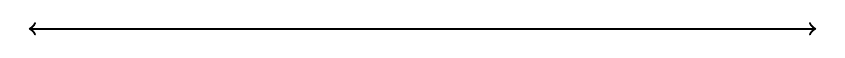
\begin{tikzpicture}
\draw[<->, thick] (-5,0)--(5,0);
\YExcoord{0}{\text{threshold}}
\color{red}\YExcoord{3}{\text{Yuan}}
\color{blue}\YExcoord{-3}{\text{Olaf}}
\end{tikzpicture}\end{center}

If I'm born before (older than) Olaf, I'm born before the threshold, so I'm old.\\
If I'm born after (younger than) Yuan I'm born after the threshold, so I'm young.
\begin{center}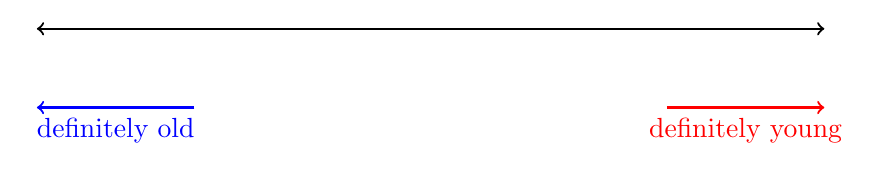
\begin{tikzpicture}
\draw[<->, thick] (-5,0)--(5,0);
\YExcoord{0}{\text{threshold}}
\color{red}\YExcoord{3}{\text{Yuan}}
\draw[->, thick] (3,-1)--(5,-1) node[midway, below]{definitely young};
\color{blue}\YExcoord{-3}{\text{Olaf}}
\draw[->, thick] (-3,-1)--(-5,-1) node[midway, below]{definitely old};
\end{tikzpicture}\end{center}
If I'm born after Olaf or before Yuan, I don't know which side of the threshold I'm on. I could be old or I could be young.
\begin{center}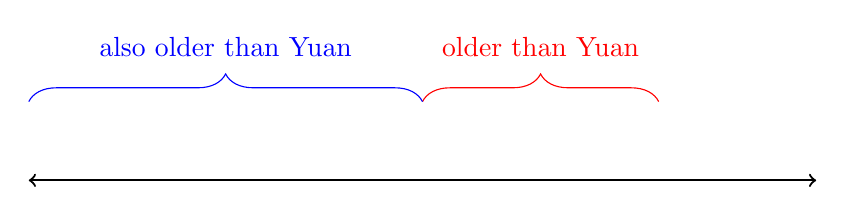
\begin{tikzpicture}
\draw[<->, thick] (-5,0)--(5,0);
\YExcoord{0}{\text{threshold}}
\color{red}\YExcoord{3}{\text{Yuan}}
\draw[decorate, decoration={brace, amplitude=10pt}] (0,1)--(3,1) node[midway, yshift=7mm]{older than Yuan};
\color{blue}\YExcoord{-3}{}
\draw[decorate, decoration={brace, amplitude=10pt}] (-5,1)--(0,1) node[midway, yshift=7mm]{also older than Yuan};
\end{tikzpicture}\end{center}
\end{solution}
%%%%%%%%%%%%%%%%%%%

\begin{question}\label{prob_s3.3:compareintuitive}
Below are graphs of two sequences with positive terms.  Assume the sequences continue as shown. Fill in the table with conclusions that can be made from the direct comparison test, if any.
\begin{center}\begin{tikzpicture}
\YEaaxis{.5}{6}{.5}{3}
\draw (6.2,0) node[shape=circle, fill=white, minimum size=4mm]{$n$};
\foreach \x in {1,...,11}
	{\draw[red] (\x/2,3/\x) node[vertex]{};
	\draw[blue] (\x/2,1/\x) node[vertex]{};}
\end{tikzpicture}\end{center}
\begin{center}\begin{tabular}{|c|c|c|}
\hline
& if $\sum\limits^{\vphantom{\frac12}} a_n$ converges & if $\sum a_n$ diverges\\[10pt]
\hline
\color{red} and if $\{a_n\}$ is the red series& \color{blue}then $\sum\limits^{\vphantom{\frac12}} b_n$ \rule{1.5cm}{1pt}& \color{blue}then $\sum b_n$ \rule{1.5cm}{1pt}\\[10pt]
\hline
\color{blue} and if $\{a_n\}$ is the blue series& \color{red}then $\sum\limits^{\vphantom{\frac12}} b_n$ \rule{1.5cm}{1pt}& \color{red}then $\sum b_n$ \rule{1.5cm}{1pt}\\[10pt]
\hline
\end{tabular}\end{center}
\end{question}
\begin{hint}
The comparison test is Theorem~\eref{CLP101}{thm:SRcomparisonTest} in the CLP-2 text. However, rather than trying to memorize which way the inequalities go in all cases, you can use the same reasoning as Question~\ref{prob_s3.3:oldies}.
\end{hint}
\begin{answer}

\begin{tabular}{|c|c|c|}
\hline
& if $\sum\limits^{\vphantom{\frac12}} a_n$ converges & if $\sum a_n$ diverges\\[10pt]
\hline
\color{red} and if $\{a_n\}$ is the red series& \color{blue}then $\sum\limits^{\vphantom{\frac12}} b_n$ CONVERGES&inconclusive \\[10pt]
\hline
\color{blue} and if $\{a_n\}$ is the blue series&inconclusive& \color{red}then $\sum\limits^{\vphantom{\frac12}} b_n$ DIVERGES\\[10pt]
\hline
\end{tabular}
\end{answer}
\begin{solution}
The comparison test is Theorem~\eref{CLP101}{thm:SRcomparisonTest} in the CLP-2 text. However, rather than trying to memorize which way the inequalities go in all cases, we  use the same reasoning as Question~\ref{prob_s3.3:oldies}.

If a sequence has positive terms, it either converges, or it diverges to infinity, with the partial sums increasing and increasing without bound. If one sequence diverges, and the other sequence is larger, then the other sequence diverges--just like being older than an old person makes you old.

If $\sum a_n$ converges, and $\{a_n\}$ is the red (larger) series, then $\sum b_n$ converges: it's smaller than a sequence that doesn't add up to infinity, so it too does not add up to infinity.

If $\sum a_n$ diverges, and $\{a_n\}$ is the blue (smaller) series, then $\sum b_n$ diverges: it's larger than a sequence that adds up to infinity, so it too adds up to infinity.

In the other cases, we can't say anything. If $\{a_n\}$ is the red (larger) series, and  $\sum a_n$ diverges, then perhaps $\{b_n\}$ behaves similarly to $\{a_n\}$ and $\sum b_n$ diverges, or perhaps $\{b_n\}$ is much, much smaller than $\{a_n\}$ and $\sum b_n$ converges.

Similarly, if $\{a_n\}$ is the blue (smaller) series, and  $\sum a_n$ converges, then perhaps $\{b_n\}$ behaves similarly to $\{a_n\}$ and $\sum b_n$ converges, or perhaps $\{b_n\}$ is much, much bigger than $\{a_n\}$ and $\sum b_n$ diverges.

\begin{center}
\begin{tabular}{|c|c|c|}
\hline
& if $\sum\limits^{\vphantom{\frac12}} a_n$ converges & if $\sum a_n$ diverges\\[10pt]
\hline
\color{red} and if $\{a_n\}$ is the red series& \color{blue}then $\sum\limits^{\vphantom{\frac12}} b_n$ CONVERGES&inconclusive \\[10pt]
\hline
\color{blue} and if $\{a_n\}$ is the blue series&inconclusive& \color{red}then $\sum\limits^{\vphantom{\frac12}} b_n$ DIVERGES\\[10pt]
\hline
\end{tabular}
\end{center}
\end{solution}
%%%%%%%%%%%%%%%%%%%
\begin{Mquestion}
For each pair of series below, decide whether the second series is a valid comparison series to determine the convergence of the first series, using the  \emph{direct} comparison test and/or the \emph{limit} comparison test.
\begin{enumerate}[(a)]
\item $\displaystyle\sum_{n=10}^{\infty} \frac{1}{n-1},$ compared to the divergent series
$\displaystyle\sum_{n=10}^{\infty} \frac{1}{n}.$
\item $\displaystyle\sum_{n=1}^{\infty} \frac{\sin n}{n^2+1},$ compared to the convergent series
$\displaystyle\sum_{n=1}^{\infty} \frac{1}{n^2}.$
\item $\displaystyle\sum_{n=5}^{\infty} \frac{n^3+5n+1}{n^6-2},$ compared to the convergent series
$\displaystyle\sum_{n=5}^{\infty} \frac{1}{n^3}.$
\item $\displaystyle\sum_{n=5}^{\infty} \frac{1}{\sqrt{n}},$ compared to the divergent series
$\displaystyle\sum_{n=5}^{\infty} \frac{1}{\sqrt[4]n}.$
\end{enumerate}
\end{Mquestion}
\begin{hint}
Think about Question~\ref{prob_s3.3:compareintuitive} to remind yourself which way the inequalities have to go for direct comparison.

Note that all the comparison series have positive terms, so we don't need to worry about that part of the limit comparison test.
\end{hint}
\begin{answer}
(a) both direct comparison and limit comparison \qquad (b) direct comparison\\
 (c) limit comparison\qquad (d) neither
\end{answer}
\begin{solution}
(a) Since $\sum \frac{1}{n}$ is divergent, we can only use it to prove series with \emph{larger} terms are divergent. This is the case here, since $\frac{1}{n-1}>\frac{1}{n}$. So, the direct comparison test is valid.

For the limit comparison test, we calculate:
\begin{align*}
\lim_{n \to \infty}\frac{a_n}{b_n}&=\lim_{n \to \infty}\frac{\frac{1}{n-1}}{\frac{1}{n}}
=\lim_{n \to \infty}\frac{1}{1-\frac{1}{n}}
=1
\end{align*}
Since the limit exists and is not zero, the limit comparison test is also valid.

(b) Since the series $\sum \frac{1}{n^2}$ converges, we can only use the direct comparison test to show the convergence of a series if its terms have \emph{smaller} absolute values. Indeed,
\[\left| \frac{\sin n}{n^2+1}\right|=\frac{|\sin n|}{n^2+1}<\frac{1}{n^2}\]
so the series are set for a direct comparison.

To check whether a limit comparison will work, we compute:
\begin{align*}
\lim_{n \to \infty}\frac{a_n}{b_n}&=\lim_{n \to \infty} \frac{\frac{\sin n}{n^2+1}}{\frac{1}{n^2}} = \lim_{n \to \infty}\frac{n^2}{n^2+1}\sin n = \lim_{n \to \infty}(1)\sin n
\end{align*}
The limit does not exist, so the limit comparison test is not a valid test to compare these two series.

(c) Since the series $\sum \frac{1}{n^3}$ converges, we can only use the direct comparison test to conclude something about a series with \emph{smaller} terms. However, \[\frac{n^3+5n+1}{n^6-2}>\frac{n^3}{n^6}=\frac{1}{n^3}.\]
Therefore the direct comparison test does not apply to this pair of series.

For the limit comparison test, we calculate:
\begin{align*}
\lim_{n \to \infty}\frac{a_n}{b_n}&=\lim_{n \to \infty}\frac{\frac{n^3+5n+1}{n^6-2}}{  \frac{1}{n^3}} = \lim_{n \to \infty}\frac{n^3+5n+1}{n^3-\frac{2}{n^3}}\left(\frac{\frac{1}{n^3}}{\frac{1}{n^3}}\right)\\
&=\lim_{n \to \infty}\frac{1+\frac{5}{n^2}+\frac{1}{n^3}}{1-\frac{2}{n^6}}=1
\end{align*}
Since the limit is a nonzero real number, we can use the limit comparison test to compare this pair of series.

(d) Since the series $\sum \frac{1}{\sqrt[4]{n}}$ diverges, we can only use the direct comparison test to show that a series with \emph{larger} terms diverges. However,
\[\frac{1}{\sqrt{n}}<\frac{1}{\sqrt[4]{n}}\]
so the direct comparison test isn't valid with this pair of series.

For the limit comparison test, we calculate:
\begin{align*}
\lim_{n \to \infty}\frac{a_n}{b_n}&=\lim_{n \to \infty}\frac{\frac{1}{\sqrt{n}}}{\frac{1}{\sqrt[4]{n}}}=\lim_{n \to \infty}\frac{1}{\sqrt[4]{n}}=0
\end{align*}
Since the limit is zero, the limit comparison test doesn't apply.
\end{solution}
%%%%%%%%%%%%%%%%%%%
\begin{question}
Suppose $a_n$ is a sequence with $\displaystyle\lim_{n \to \infty}a_n = \frac{1}{2}$. Does $\displaystyle\sum_{n=7}^\infty a_n$ converge or diverge, or is it not possible to determine this from the information given? Why?
\end{question}
\begin{hint}
The divergence test is Theorem~\eref{CLP101}{thm:SRdivergenceTest} in the CLP-2 text.
\end{hint}
\begin{answer}
It diverges by the divergence test, because $\displaystyle\lim_{n \to \infty}a_n \neq 0$.
\end{answer}
\begin{solution}
It diverges by the divergence test, because $\displaystyle\lim_{n \to \infty}a_n \neq 0$.
\end{solution}
%%%%%%%%%%%%%%%%%%%



%%%%%%%%%%%%%%%%%%
\begin{Mquestion}
What flaw renders the following reasoning invalid?
\begin{quote}\color{blue}
Q: Determine whether $\displaystyle\sum_{n=1}^\infty \dfrac{\sin n}{n}$ converges or diverges.\\
A: First, we will evaluate $\displaystyle\lim_{n \to \infty} \dfrac{\sin n}{n}$.
\begin{itemize}
\item Note $\dfrac{-1}{n} \leq \dfrac{\sin n}{n} \leq \dfrac{1}{n}$ for $n \ge 1$.
\item Note also that $\displaystyle\lim_{n \to \infty}\frac{-1}{n}=\displaystyle\lim_{n \to \infty}\frac{1}{n}=0$.
\item Therefore, by the Squeeze Theorem, $\displaystyle\lim_{n \to \infty} \dfrac{\sin n}{n}=0$ as well.
\end{itemize}
So, by the divergence test, $\displaystyle\sum_{n=1}^\infty \dfrac{\sin n}{n}$ converges.
\end{quote}
\end{Mquestion}
\begin{hint}
The limit is calculated correctly.
\end{hint}
\begin{answer}
We cannot use the divergence test to show that a series converges. It is inconclusive in this case.
\end{answer}
\begin{solution}
 The divergence test (Theorem~\eref{CLP101}{thm:SRdivergenceTest} in the CLP-2 text) is inconclusive when $\displaystyle\lim_{n \to \infty}a_n=0$. We cannot use the divergence test to show that a series converges.
\end{solution}



%%%%%%%%%%%%%%%%%%
\begin{question}
What flaw renders the following reasoning invalid?
\begin{quote}\color{blue}
Q: Determine whether $\displaystyle\sum_{n=1}^\infty \left(\sin(\pi n)+2\right)$ converges or diverges.\\
A: We use the integral test. Let $f(x)=\sin(\pi x)+2$. Note $f(x)$ is always positive, since $\sin(x)+2 \geq -1+2 =1$. Also, $f(x)$ is continuous.
\begin{align*}
\int_1^\infty [\sin(\pi x)+2] dx &= \lim_{b \to \infty}\int_1^b [\sin(\pi x)+2 ]dx\\
&=\lim_{b \to \infty} \left[\left.-\frac{1}{\pi}\cos(\pi x)+2x \right|_1^b\right]\\
&=\lim_{b \to \infty}\left[ -\frac{1}{\pi}\cos(\pi b)+2b +\frac{1}{\pi}(-1)-2\right]\\
&=\infty
\end{align*}
By the integral test, since the integral diverges, also $\displaystyle\sum_{n=1}^\infty\left(  \sin(\pi n)+2\right)$ diverges.
\end{quote}
\end{question}
\begin{hint}
It is true that $f(x)$ is positive. What else has to be true of $f(x)$ for the integral test to apply?
\end{hint}
\begin{answer}
The integral test does not apply because $f(x)$ is not decreasing.
\end{answer}
\begin{solution}
The integral test does not apply because $f(x)$ is not decreasing.
\end{solution}




%%%%%%%%%%%%%%%%%%
\begin{question}
What flaw renders the following reasoning invalid?
\begin{quote}\color{blue}
Q: Determine whether the series
$\displaystyle\sum_{n=1}^\infty \dfrac{2^{n+1}n^2}{e^n+2n}$
converges or diverges.\\
A: We want to compare this series to the series $\displaystyle\sum_{n=1}^\infty \dfrac{2^{n+1}}{e^n}$. Note both this series and the series in the question have positive terms.

First, we find that $\dfrac{2^{n+1}n^2}{e^n+2n} > \dfrac{2^{n+1}}{e^n}$ when $n$ is sufficiently large. The justification for this claim is as follows:
\begin{itemize}
\item We note that $e^n(n^2-1)>n^2-1>2n$ for $n$ sufficiently large.
\item Therefore, $e^n \cdot n^2 > e^n+2n$
\item Therefore, $2^{n+1}\cdot e^n \cdot n^2 > 2^{n+1}(e^n+2n)$
\item Since $e^n+2n$ and $e^n$ are both expressions that work out to be positive for the values of $n$ under consideration, we can divide both sides of the inequality by these terms without having to flip the inequality. So,
$\dfrac{2^{n+1}n^2}{e^n+2n}>\dfrac{2^{n+1}}{e^n}$.
\end{itemize}
Now, we claim  $\displaystyle\sum_{n=1}^\infty \dfrac{2^{n+1}}{e^n}$ converges.\\
 Note  $\displaystyle\sum_{n=1}^\infty \dfrac{2^{n+1}}{e^n}= 2\displaystyle\sum_{n=1}^\infty \dfrac{2^{n}}{e^n}= 2\displaystyle\sum_{n=1}^\infty \left(\dfrac{2}{e}\right)^n$. This is a geometric series with $r=\frac{2}{e}$. Since $2/e <1$, the series converges.

 Now, by the Direct Comparison Test, we conclude that $\displaystyle\sum_{n=1}^\infty \dfrac{2^{n+1}n^2}{e^n+2n}$ converges.
 \end{quote}
\end{question}
\begin{hint}
Refer to Question~\ref{prob_s3.3:compareintuitive}.
\end{hint}
\begin{answer}
The inequality goes the wrong way, so the direct comparison test (with this comparison series) is inconclusive.
\end{answer}
\begin{solution}
The inequality goes the wrong way, so the direct comparison test (with this comparison series) is inconclusive.
\end{solution}


\begin{question}
Which of the series below are alternating?

\hfill(A) $\displaystyle\sum_{n=1}^\infty \sin n$\hfill
(B) $\displaystyle\sum_{n=1}^\infty \frac{\cos(\pi n)}{n^3}$\hfill
(C) $\displaystyle\sum_{n=1}^\infty \frac{7}{(-n)^{2n}}$\hfill
(D) $\displaystyle\sum_{n=1}^\infty \frac{(-2)^n}{3^{n+1}}$\hfill~
\end{question}
\begin{hint}
The definition of an alternating series is given in the start of Section~\eref{CLP101}{sec:AST}
 in the CLP-2 text.
\end{hint}
\begin{answer}
(B), (D)
\end{answer}
\begin{solution}
Although the terms of (A) are sometimes negative and sometimes positive, they are not strictly alternating in a  positive-negative-positive-negative pattern. For instance, $\sin 1$ and $\sin 2$ are both postive. So, (A) is not an alternating series.

When $n$ is a whole number, $\cos(\pi n) = (-1)^n$, so (B) is alternating.

Since the exponent of $(-n)$ in (C) is even, the terms are always positive. Therefore (C) is not alternating.

(D) is an alternating series.
\end{solution}

%%%%%%%%%%%%%%%%%%%
\begin{Mquestion}
Give an example of a convergent series for which the ratio test is inconclusive.
\end{Mquestion}
\begin{hint}
For the ratio test to be inconclusive, $\lim\limits_{n \to \infty}\left|\dfrac{a_{n+1}}{a_n}\right|$ should be 1 or nonexistent.
\end{hint}
\begin{answer}
One possible answer: $\displaystyle\sum_{n=1}^\infty \dfrac{1}{n^2}$.
\end{answer}
\begin{solution}
One possible answer: $\displaystyle\sum_{n=1}^\infty \dfrac{1}{n^2}$. This series converges (it's a $p$--series with $p=2>1$), but if we take the ratio of consecutive terms:
\[\lim_{n \to \infty}\frac{a_{n+1}}{a_n} = \lim_{n \to \infty}\frac{n^2}{(n+1)^2}=1\]
The limit of the ratio is 1, so the ratio test is inconclusive.
\end{solution}
%%%%%%%%%%%%%%%%%%%
\begin{question}
Imagine you're taking an exam, and you momentarily forget exactly how the inequality in the ratio test works. You remember there's a ratio, but you don't remember which term goes on top; you remember there's something about the limit being greater than or less than one, but you don't remember which way implies convergence.

 Explain why
\[\lim_{n \to \infty}\left|\frac{a_{n+1}}{a_{n}}\right|>1\]
or, equivalently,
\[\lim_{n \to \infty}\left|\frac{a_n}{a_{n+1}}\right|<1\]
should mean that the sum $\sum\limits_{n=1}^\infty a_n$ \emph{diverges} (rather than converging).
\end{question}
\begin{hint}
By the divergence test, for a series $\sum a_n$ to \emph{converge}, we need $\lim\limits_{n \to \infty} a_n=0$. That is, the magnitude (absolute value) of the terms needs to be getting smaller.
\end{hint}
\begin{answer}
By the divergence test, for a series $\sum a_n$ to \emph{converge}, we need $\lim\limits_{n \to \infty} a_n=0$. That is, the magnitude (absolute value) of the terms needs to be getting smaller. If $\displaystyle\lim_{n \to \infty}\left|\frac{a_n}{a_{n+1}}\right|<1$ or (equivalently) $\displaystyle \lim_{n \to \infty}\left|\frac{a_{n+1}}{a_{n}}\right|>1$, then $|a_{n+1}|>|a_n|$ for sufficiently large $n$, so the terms are actually \emph{growing} in magnitude. That means the series diverges, by the divergence test.
\end{answer}
\begin{solution}
By the divergence test, for a series $\sum a_n$ to \emph{converge}, we need $\lim\limits_{n \to \infty} a_n=0$. That is, the magnitude (absolute value) of the terms needs to be getting smaller. If $\displaystyle\lim_{n \to \infty}\left|\frac{a_n}{a_{n+1}}\right|<1$ or (equivalently) $\displaystyle \lim_{n \to \infty}\left|\frac{a_{n+1}}{a_{n}}\right|>1$, then $|a_{n+1}|>|a_n|$ for sufficiently large $n$, so the terms are actually \emph{growing} in magnitude. That means the series diverges, by the divergence test.
\end{solution}

%%%%%%%%%%%%%%%%%%%
\begin{question}
Give an example of a series $\displaystyle\sum_{n=a}^\infty a_n$, with a function $f(x)$ such that $f(n)=a_n$ for all whole numbers $n$, such that:
\begin{itemize}
\item $\displaystyle\int_a^\infty f(x)\,\dee{x}$ diverges, while
\item $\displaystyle\sum_{n=a}^\infty a_n$ converges.
\end{itemize}
\end{question}
\begin{hint}
If $f(x)$ is positive and decreasing, then the integral test tells you that the integral and the series either both increase or both decrease. So, in order to find an example with the properties required in the question, you need $f(x)$ to \emph{not} be both positive and decreasing.
\end{hint}
\begin{answer}
One possible answer: $f(x) = \sin(\pi x)$, $a_n=0$ for every $n$.

By the integral test, any answer will use a function $f(x)$  that is \emph{not} both positive and decreasing.
\end{answer}
\begin{solution}
The terms of the series only see a small portion of the domain of the integral. We can try to think of a function $f(x)$ that behaves ``nicely" when $x$ is a whole number (that is, it produces a sequence whose sum converges), but is more unruly when $x$ is not a whole number.

For example, suppose $f(x)=\sin(\pi x)$. Then $f(x)=0$ for every integer $x$, but this is not representative of the function as a whole. Indeed, our corresponding series has terms $\{a_n\}=\{0,0,0,\ldots\}$.
\begin{itemize}
\item $\displaystyle\int_{1}^\infty \sin(\pi x)\,\dee{x} = \lim_{R \to \infty} \left[-\frac{1}{\pi}\cos (\pi x)\right]_1^R = \lim_{R \to \infty}\Big[-\cos (\pi R)\Big]-\frac{1}{\pi}$\\
 Since the limit does not exist, the integral diverges.
 \item $\displaystyle\sum_{n=1}^{\infty}\sin(\pi n) = \sum_{n=1}^\infty 0 = 0$. The series converges.
\end{itemize}\end{solution}
%%%%%%%%%%%%%%%%%%%

\begin{question}[2016Q5]
Suppose that you want to use the Limit Comparison Test on the series
$ \displaystyle \sum_{n=0}^{\infty} a_n$ where\linebreak $\displaystyle a_n = \frac{2^n+n}{3^n+1}$.
Write down a sequence $\{b_n\}$ such that $\displaystyle \lim\limits_{n\to\infty} \frac{a_n}{b_n}$
exists and is nonzero. (You don't have to carry out the Limit Comparison Test)
\end{question}

\begin{hint}
Review  Theorem \eref{CLP101}{thm:SRlimitComparison} and
Example \eref{CLP101}{eg:SRlimCompA} in the CLP-2 text.

\end{hint}

\begin{answer}
One possible answer:
$b_n=\displaystyle \frac{2^n}{3^n}$
\end{answer}

\begin{solution}
When $n$ is very large, the term $2^n$ dominates the numerator,
and the term $3^n$ dominates the denominator.  So when $n$ is very large
$a_n\approx   \frac{2^n}{3^n}$. Therefore we should  take $b_n=\displaystyle \frac{2^n}{3^n}$.
Note that, with this choice of $b_n$,
\begin{align*}
 \lim_{n\to\infty} \frac{a_n}{b_n}
= \lim_{n\to\infty} \frac{2^n+n}{3^n+1}\ \frac{3^n}{2^n}
= \lim_{n\to\infty} \frac{1+ n/2^{n}}{1+1/3^{n}}
=1
\end{align*}
as desired.
\end{solution}

%%%%%%%%%%%%%%%%%%%%%%%%%%%%%%%%%%5
\begin{Mquestion}[2014D, 2016A]
Decide whether each of the following statements is true or false.
If false, provide a counterexample. If true provide a brief justification.

\begin{enumerate}[(a)]
\item
If $\displaystyle\lim_{n\rightarrow\infty}a_n=0$,
               then $\sum\limits_{n=1}^{\infty} a_n$ converges.
\item
 If $\displaystyle\lim_{n\rightarrow\infty}a_n=0$,
               then $\sum\limits_{n=1}^{\infty} (-1)^{n\mathstrut} a_n$ converges.
\item
If $0\le a_n \le b_n$ and $\sum\limits_{n=1}^{\infty} b_n$ diverges,
then $\sum\limits_{n=1}^{\infty} a_n$ diverges.
\end{enumerate}
\end{Mquestion}

\begin{hint}
Don't jump to conclusions about properties of the $a_n$'s.
\end{hint}

\begin{answer}
(a) In general false. The harmonic series $\sum\limits_{n=1}^\infty\frac{1}{n}$
provides a counterexample.

\noindent (b)
In general false. If $a_n =(-1)^n\frac{1}{n}$, then
$\sum\limits_{n=1}^{\infty} (-1)^{n\mathstrut} a_n$ is again the harmonic series
$\sum_{n=1}\limits^\infty\frac{1}{n}$, which diverges.

\noindent (c)
In general false. Take, for example, $a_n=0$ and $b_n=1$.

\end{answer}

\begin{solution} (a)
In general false. The harmonic series $\sum\limits_{n=1}^\infty\frac{1}{n}$
diverges by the $p$--test with $p=1$.


\noindent (b)
Be careful. You were not told that the $a_n$'s are positive. So this is false in general.
If $a_n =(-1)^n\frac{1}{n}$, then
$\sum\limits_{n=1}^{\infty} (-1)^{n\mathstrut} a_n$ is again the harmonic series
$\sum\limits_{n=1}^\infty\frac{1}{n}$, which diverges.

\noindent (c)
In general false. Take, for example, $a_n=0$ and $b_n=1$.

\end{solution}
%%%%%%%%%%%%%%%%%%%




%%%%%%%%%%%%%%%%%%
\subsection*{\Procedural}
%%%%%%%%%%%%%%%%%%

\begin{question}[2016Q5]
Does the series $\displaystyle \sum_{n=2}^\infty \frac{n^2}{3n^2+\sqrt n}$ converge?
\end{question}

\begin{hint}
Always try the divergence test first (in your head).
\end{hint}

\begin{answer}
No. It diverges.
\end{answer}

\begin{solution}
First, we'll check the divergence test. It doesn't always work, but if it does, it's likely the easiest path.
\begin{align*}
\lim_{n\to\infty} \frac{n^2}{3n^2+\sqrt n} \left(\frac{\frac{1}{n^2}}{\frac{1}{n^2}}\right)
 =  \lim_{n\to\infty} \frac{1}{3+\frac{1}{n\sqrt n}}
 = \frac{1}{3}
 \neq 0
\end{align*}
Since the limit of the terms being added is not zero, the series diverges by the divergence test.
\end{solution}

%%%%%%%%%%%%%%%%%%%%%%%%%%%%%%

\begin{question}[2014D]
Determine, with explanation, whether the series
$\displaystyle \sum_{n=1}^\infty \frac{5^k}{4^k+3^k}$ converges
or diverges.
\end{question}

\begin{hint}
Which test should you always try first (in your head)?
\end{hint}

\begin{answer}
It diverges.
\end{answer}

\begin{solution}
This precise question was asked on a 2014 final exam. Note that the
$n^{\rm th}$ term in the series is $a_n=\frac{5^k}{4^k+3^k}$ and does
\emph{not} depend on $n$! There are two possibilities. Either this was
intentional (and the instructor was being particularly nasty) or it was a
typo and the intention was to have $a_n=\frac{5^n}{4^n+3^n}$. In both cases,
the limit
\begin{align*}
\lim_{n\to\infty} a_n
&=\lim_{n\to\infty} \frac{5^k}{4^k+3^k}
 = \frac{5^k}{4^k+3^k}
 \neq 0 \\
\lim_{n\to\infty} a_n
&=\lim_{n\to\infty} \frac{5^n}{4^n+3^n}
=\lim_{n\to\infty} \frac{(5/4)^n}{1+(3/4)^n}
 = +\infty
 \neq 0 \\
\end{align*}
is nonzero,  so the series diverges by the divergence test.
\end{solution}

%%%%%%%%%%%%%%%%%%%%%%%%%%%%%%%
\begin{Mquestion}[2016Q5]
Determine whether the series
$\displaystyle\sum_{n=0}^\infty\frac{1}{n+\frac{1}{2}}$
is convergent or divergent. If it is convergent, find its value.
\end{Mquestion}

\begin{hint}
Review the integral test, which is
Theorem \eref{CLP101}{thm:SRintegralTest} in the CLP-2 text.
\end{hint}

\begin{answer}
The series diverges.
\end{answer}

\begin{solution}
We usually check the divergence test first, to look for low-hanging fruit. The limit of the terms being added is zero:
\[\lim_{n \to \infty}\frac{1}{n+\frac{1}{2}}=0\]
so the divergence test is inconclusive. That is, we need to look harder.

Next, we might consider a comparison test--these can also provide us (if we're lucky) with an easy path. The terms we're adding look somewhat like $\frac{1}{n}$, but our terms are \emph{smaller} than these terms, which form the terms of the \emph{divergent} harmonic series. So, a direct comparison seems unlikely. Now we search for more exotic tests.

Let $\displaystyle f(x) =\frac{1}{x+\frac{1}{2}}$.
Note $f(x)$ is positive and decreases as $x$ increases.
So, by the integral test, which is
Theorem \eref{CLP101}{thm:SRintegralTest} in the CLP-2 text,
the given series converges if and only if the
integral $\int_0^\infty\frac{1}{x+\frac{1}{2}} \,\dee{x}$ converges.
Since
\begin{align*}
\int_0^\infty \frac{1}{x+\frac{1}{2}} \,\dee{x} =
\lim_{R\rightarrow\infty} \int_0^R\frac{1}{x+\frac{1}{2}} \,\dee{x}
&=\lim_{R\rightarrow\infty} \bigg[ \log\Big(x+\frac{1}{2}\Big)\bigg]^{x=R}_{x=0} \\
&=\lim_{R\to\infty} \bigg[ \log\Big(R+\frac{1}{2}\Big) - \log\frac12 \bigg]
\end{align*}
diverges, the series diverges.
\end{solution}

%%%%%%%%%%%%%%%%%%%





\begin{Mquestion}
Does the following series converge or diverge?
$\displaystyle\sum_{k=1}^\infty\frac{1}{\sqrt{k}\sqrt{k+1}}$
\end{Mquestion}

\begin{hint}
A comparison might be helpful--try some algebraic manipulation to find a likely series to compare it to.
\end{hint}

\begin{answer}
It diverges.
\end{answer}

\begin{solution}
The terms of the series tend to 0, so we can't use the divergence test.

To generate a guess about its convergence, we do the following:
\[\sum \frac{1}{\sqrt{k}\sqrt{k+1}}=\sum\frac{1}{\sqrt{k^2+k}} \approx \sum\frac{1}{\sqrt{k^2}}=\sum\frac{1}{k}\]We guess that our series behaves like the harmonic series, and the harmonic series diverges (which can be demonstrated by $p$-test or integral test). So, we guess that our series diverges. However, in order to directly compare our series to the harmonic series and show our series diverges, our terms would have to be \emph{bigger} than the terms in the harmonic series, and this is not the case. So, we use limit comparison.

\begin{align*}
\frac{\frac{1}{k}}{\frac{1}{\sqrt{k^2+k}}}&=\frac{\sqrt{k^2+k}}{k}=\frac{\sqrt{k^2+k}}{\sqrt{k^2}}=
\sqrt{\frac{k^2+k}{k^2}}=\sqrt{1+\frac{1}{k}},\mbox{ so}\\
\lim_{k \rightarrow \infty}\frac{\frac{1}{k}}{\frac{1}{\sqrt{k^2+k}}}&=\lim_{k \rightarrow \infty}\sqrt{1+\frac{1}{k}}=1
\end{align*}

Since 1 is a real number greater than 0, by the Limit Comparison Test, $\sum \frac{1}{\sqrt{k}\sqrt{k+1}}$  diverges, like $\sum \frac{1}{k}$.
\end{solution}








%%%%%%%%%%%%%%%%%%%




\begin{question}
Evaluate the following series, or show that it diverges:
$\displaystyle\sum_{k=30}^\infty 3(1.001)^k$.
\end{question}

\begin{hint}
This is a geometric series.
\end{hint}

\begin{answer}
This is a geometric series with $r=1.001$. Since $|r|>1$, it is divergent.
\end{answer}

\begin{solution}
This is a geometric series with $r=1.001$. Since $|r|>1$, it is divergent.
\end{solution}








%%%%%%%%%%%%%%%%%%%




\begin{Mquestion}
Evaluate the following series, or show that it diverges:
$\displaystyle\sum_{n=3}^\infty \left(\frac{-1}{5}\right)^n$.
\end{Mquestion}

\begin{hint}
Notice that the series is geometric, but it doesn't start at $n=0$.
\end{hint}

\begin{answer}
The series converges to $-\dfrac{1}{150}$.
\end{answer}

\begin{solution}
This is a geometric series with $r=\frac{-1}{5}$. Since $|r|<1$, it is convergent.

We want to use the formula $\sum_{n=0}^\infty r^n=\frac{1}{1-r}$, but our series does not start at 0, so we re-write it:
\begin{align*}
\sum_{n=3}^\infty \left(\frac{-1}{5}\right)^n&=
\sum_{n=0}^\infty \left(\frac{-1}{5}\right)^n-
\sum_{n=0}^2 \left(\frac{-1}{5}\right)^n
=\frac{1}{1-(-1/5)} - \left(1-\frac{1}{5}+\frac{1}{25} \right)\\
&=\frac{1}{6/5}-1+\frac{1}{5}-\frac{1}{25}
=
\frac{5}{6}+\frac{-25+5-1}{25}=-\frac{1}{150}
\end{align*}
\end{solution}








%%%%%%%%%%%%%%%%%%%

\begin{question}
Does the following series converge or diverge?
$\displaystyle\sum_{n=7}^\infty \sin(\pi n)$
\end{question}

\begin{hint}
Note $n$ only takes integer values: what's $\sin(\pi n)$ when $n$ is an integer?
\end{hint}

\begin{answer}
The series converges.
\end{answer}

\begin{solution}
For any integer $n$, $\sin(\pi n)=0$, so
$\sum \sin(\pi n)=\sum 0 = 0$. So, this series converges.
\end{solution}


%%%%%%%%%%%%%%%%%%%

\begin{question}
Does the following series converge or diverge?
$\displaystyle\sum_{n=7}^\infty\cos(\pi n)$
\end{question}

\begin{hint}
Note $n$ only takes integer values: what's $\cos(\pi n)$ when $n$ is an integer?
\end{hint}

\begin{answer}
It diverges.
\end{answer}

\begin{solution}
For any integer $n$, $\cos(\pi n)=\pm 1$, so
$\lim\limits_{n \rightarrow \infty}\cos(\pi n) \neq 0$. \\
By the divergence test, this series diverges.
\end{solution}
%%%%%%%%%%%%%%%%%%%




\begin{Mquestion}
Does the following series converge or diverge?
$\displaystyle\sum_{k=1}^\infty \frac{e^k}{k!}$.
\end{Mquestion}

\begin{hint}
What's the test that you should always think of when you see a factorial?
\end{hint}

\begin{answer}
The series converges.
\end{answer}

\begin{solution}
Factorials grow super fast. Like, wow, really fast. Even faster than exponentials. So the terms are going to zero, and the divergence test won't help us. Let's use ratio--it's a good go-to test with factorials.
\begin{align*}
\frac{a_{k+1}}{a_k}&=\frac{\frac{e^{k+1}}{(k+1)!}}{\frac{e^k}{k!}}=\frac{e^{k+1}}{e^k}\cdot\frac{k!}{(k+1)!}
=
e\cdot\frac{k(k-1)\cdots(1)}{(k+1)(k)(k-1)\cdots(1)}=e\cdot\frac{1}{k+1}=\frac{e}{k+1}
\intertext{Since $e$ is a constant,}
\lim_{k \rightarrow \infty}\frac{a_{k+1}}{a_k}&=\lim_{k \rightarrow \infty}\frac{e}{k+1}=0
\end{align*}
Since $0<1$, by the  ratio test, the series converges.
\end{solution}








%%%%%%%%%%%%%%%%%%%




\begin{question}
Evaluate the following series, or show that it diverges:
$\displaystyle\sum_{k=0}^\infty\frac{2^k}{3^{k+2}}$.
\end{question}

\begin{hint}
This is a geometric series, but you'll need to do a little algebra to figure out $r$.
\end{hint}

\begin{answer}
The series converges to $\dfrac{1}{3}$.
\end{answer}

\begin{solution}
This is close to being in the form of a geometric series. First, we should have our powers be $k$, not $k+2$, but we notice $3^{k+2}=3^k3^2=9\cdot3^2$, so:
\begin{align*}
\sum_{k=0}^\infty\frac{2^k}{3^{k+2}}&=\sum_{k=0}^\infty\frac{2^k}{9\cdot3^k}
=\frac{1}{9}\sum_{k=0}^\infty\frac{2^k}{3^k}=\frac{1}{9}\sum_{k=0}^\infty\left(\frac{2}{3}\right)^k
\intertext{Now it looks like a geometric series with $r=\frac{2}{3}$}
&=\frac{1}{9}\left(\frac{1}{1-(2/3)}\right)=\frac{1}{3}
\end{align*}
In conclusion: this (geometric) series is convergent, and its sum is $\dfrac{1}{3}$.
\end{solution}








%%%%%%%%%%%%%%%%%%%





\begin{question}
Does the following series converge or diverge?
$\displaystyle\sum_{n=1}^\infty\frac{n!n!}{(2n)!}$.
\end{question}

\begin{hint}
Which test fits most often with factorials?
\end{hint}

\begin{answer}
The series converges.
\end{answer}

\begin{solution}
Usually with factorials, we want to use the divergence test or the ratio test. Since the terms are indeed tending towards zero, we are left with the ratio test.
\begin{align*}
\frac{a_{n+1}}{a_n}&=\frac{\frac{(n+1)!(n+1)!}{(2n+2)!}}{\frac{n!n!}{(2n)!}}=\frac{(n+1)!(n+1)!}{n!n!}\cdot\frac{(2n)!}{(2n+2)!}\\
&=\tfrac{\textcolor{red}{(n+1)}{(n)}{(n-1)}\cdots{(1)}}{{n}{(n-1)}\cdots{(1)}}
\cdot\tfrac{\textcolor{red}{(n+1)}{(n)}{(n-1)}\cdots{(1)}}{{n}{(n-1)}\cdots{(1)}}
\cdot
\tfrac{{(2n)}{(2n-1)}{(2n-2)}\cdots{(1)}}{\textcolor{red}{(2n+2)(2n+1)}{(2n)}{(2n-1)}{(2n-2)}\cdots{(1)}}
\\
&=(n+1)(n+1) \cdot \frac{1}{(2n+2)(2n+1)}\mbox{, so}\\
\lim_{n \rightarrow \infty}\frac{a_{n+1}}{a_n}&=\lim_{n \rightarrow \infty}\frac{(n+1)(n+1)}{(2n+2)(2n+1)}
=\lim_{n \rightarrow \infty}\frac{(n+1)(n+1)}{2(n+1)(2n+1)}
=\lim_{n \rightarrow \infty}\frac{n+1}{4n+2}=\frac{1}{4}
\end{align*}
Since the limit is a number less than 1, the series converges by the ratio test.
\end{solution}








%%%%%%%%%%%%%%%%%%%




\begin{Mquestion}
Does the following series converge or diverge?
$\displaystyle\sum_{n=1}^\infty\frac{n^2+1}{2n^4+n}$.
\end{Mquestion}

\begin{hint}
Try finding a nice comparison.
\end{hint}

\begin{answer}
It converges.
\end{answer}

\begin{solution}
We want to make an estimation, when $n$ gets big:
\[\frac{n^2+1}{2n^4+n} \approx \frac{n^2}{2n^4}=\frac{1}{2n^2}\]
Since $\sum \frac{1}{2n^2}$ is a convergent series (by $p$-test, or integral test), we guess that our series is convergent as well. If we wanted to use comparison test, we should have to show $\frac{n^2+1}{2n^4+n}<\frac{1}{2n^2}$, which seems unpleasant, so let's use limit comparison.

\[\lim_{n \rightarrow \infty}\frac{\frac{n^2+1}{2n^4+n}}{\frac{1}{2n^2}}=\lim_{n \rightarrow \infty}\frac{(n^2+1)2n^2}{2n^4+n}
=\lim_{n \rightarrow \infty}\frac{2n^4+2n^2}{2n^4+n}\left(\frac{1/n^4}{1/n^4}\right)=\lim_{n \rightarrow \infty}\frac{2+\frac{2}{n^2}}{2+\frac{1}{n^3}}=1
\]

Since the limit is a positive finite number, by the Limit Comparison Test, $\sum \frac{n^1+1}{2n^4+n}$ does the same thing $\sum\frac{1}{2n^2}$ does: it converges.
\end{solution}


%%%%%%%%%%%%%%%%%%%%%%%%%%%%%
\begin{Mquestion}[2016Q5]
Show that the series $\displaystyle\sum_{n=3}^\infty \frac{5}{n(\log n)^{3/2}}$ converges.
\end{Mquestion}

\begin{hint}
With the substitution $u=\log x$, the function $\dfrac{1}{x(\log x)^{3/2}}$ is easily integrable.
\end{hint}

\begin{answer}
Let $\displaystyle f(x) = \frac{5}{x(\log x)^{3/2}}$.
Then $f(x)$ is positive and decreases as $x$ increases.
So the sum $\displaystyle\sum_3^{\infty} f(n)$ and the
integral $\displaystyle\int_3^\infty f(x) \,\dee{x}$
either both converge or both diverge, by the integral test, which is
Theorem \eref{CLP101}{thm:SRintegralTest} in the CLP-2 text.
For the integral, we use the substitution
$u = \log x$, $\dee{u} = \frac{\dee{x}}{x}$ to get
\begin{align*}
\int_3^\infty \frac{5 \,\dee{x}}{x(\log x)^{3/2}} = \int_{\log 3}^\infty \frac{5 \,\dee{u}}{u^{3/2}}
\end{align*}
which converges by the $p$--test (which is
Example \eref{CLP101}{eg:IMPp1} in the CLP-2 text)
with $p=\frac{3}{2} > 1$.
\end{answer}

\begin{solution}
First, we rule out some of the easier tests. The limit of the terms being added is zero, so the divergence test is inconclusive. The terms being added are smaller than the terms of the (divergent) harmonic series, $\sum \frac{1}{n}$, so we can't directly compare these two series, and there isn't another obvious  series to compare ours to. However, the terms being added seem like a function we could integrate.

Let $\displaystyle f(x) = \frac{5}{x(\log x)^{3/2}}$.
Then $f(x)$ is positive and decreases as $x$ increases.
So the sum $\displaystyle\sum_3^{\infty} f(n)$ and the
integral $\displaystyle\int_3^\infty f(x) \,\dee{x}$
either both converge or both diverge, by the integral test, which is
Theorem \eref{CLP101}{thm:SRintegralTest} in the CLP-2 text.
For the integral, we use the substitution
$u = \log x$, $\dee{u} = \frac{\dee{x}}{x}$ to get
\begin{align*}
\int_3^\infty \frac{5 \,\dee{x}}{x(\log x)^{3/2}} = \int_{\log 3}^\infty \frac{5 \,\dee{u}}{u^{3/2}}
\end{align*}
which converges by the $p$--test (which is
Example \eref{CLP101}{eg:IMPp1} in the CLP-2 text)
with $p=\frac{3}{2} > 1$.
\end{solution}

%%%%%%%%%%%%%%%%%%%%%%%%%%%%
\begin{question}[2014A]
Find the values of $p$ for which the series
$\displaystyle{\sum_{n=2}^\infty \frac{1}{n(\log n)^p}}$ converges.
\end{question}

\begin{hint}
Combine the integral test with the results about $p$-series, Example~\eref{CLP101}{eg:SRpTest}
 in the CLP-2 text.
\end{hint}

\begin{answer}
$p>1$
\end{answer}

\begin{solution}
Let $f(x)=\frac{1}{x(\log x)^p}$. Then $f(x)$ is positive for $n \ge 3$, and $f(x)$ decreases as $x$ increases. So, we can use the integral test,
Theorem \eref{CLP101}{thm:SRintegralTest} in the CLP-2 text.

\begin{align*}
\int_2^\infty\!\! \frac{1}{x(\log x)^p} \dee{x}
&=\lim_{R\rightarrow\infty}\int_2^R\!\! \frac{1}{(\log x)^p} \frac{\dee{x}}{x}
=\lim_{R\rightarrow\infty}\int_{\log 2}^{\log R}\!\! \frac{1}{u^p} \dee{u}
\quad\text{with $u=\log x$, $\dee{u}=\frac{\dee{x}}{x}$} \\
\end{align*}
Using the results about $p$-series, Example~\eref{CLP101}{eg:SRpTest} in the CLP-2 text,
we know this integral converges if and only if $p>1$, so the same is true for the
series by the integral test.
\end{solution}
%%%%%%%%%%%%%%%%%%%

\begin{Mquestion}[2016A]
Does ${\displaystyle\sum_{n=1}^\infty\frac{e^{-\sqrt{n}}}{\sqrt{n}}}$ converge or diverge?
\end{Mquestion}

\begin{hint}
Try the substitution $u=\sqrt{x}$.
\end{hint}

\begin{answer}
It converges.
\end{answer}

\begin{solution}
As usual, let's see whether the ``easy" tests work. The terms we're adding converge to zero:
\[\lim_{n \to \infty}\frac{e^{-\sqrt{n}}}{\sqrt{n}}=\lim_{n \to \infty}\frac{1}{\sqrt{n}e^{\sqrt{n}}}=0 \]
so the divergence test is inconclusive. Our series isn't geometric, and it doesn't seem obvious how to compare it to a geometric series. However, the terms we're adding seem like they would make an integrable function.

Set $f(x)=\frac{e^{-\sqrt{x}}}{\sqrt{x}}$. For $x\ge1$,
this function is positive and decreasing (since it is the product of
the two positive decreasing functions $e^{-\sqrt x}$ and $\frac1{\sqrt x}$).
We use the integral test with this function.
Using the substitution $u=\sqrt x$, so that
$\dee{u} = \frac1{2\sqrt x}\,\dee{x}$, we see that
\begin{align*}
\int_1^\infty f(x)\,\dee{x}
&=\lim_{R\rightarrow\infty}\int_1^R \bigg( \frac{e^{-\sqrt{x}}}{\sqrt{x}}\,\dee{x} \bigg) \\[0.05in]
&=\lim_{R\rightarrow\infty} \bigg( \int_1^{\sqrt{R}} e^{-u}\cdot2\,\dee{u} \bigg) \\[0.05in]
&=\lim_{R\rightarrow\infty} \bigg( {-}2e^{-u}\Big|_1^{\sqrt{R}} \bigg) \\[0.05in]
&=\lim_{R\rightarrow\infty} \bigg( {-}2e^{-\sqrt R} + 2e^{-\sqrt1} \bigg)
= 0 + 2e^{-1},
\end{align*}
and so this improper integral converges. By the integral test,
the given series also converges.
\end{solution}
%%%%%%%%%%%%%%%%%%%


\begin{question}[2016Q6]
Use the comparison test (not the limit comparison test) to show whether the series \\
$\displaystyle \sum_{n=2}^{\infty} \frac{\sqrt{3 n^2 - 7}}{n^{3}}$ converges or diverges.
\end{question}

\begin{hint}
Review Example \eref{CLP101}{eg:SRcomparisonTestA} in the
CLP-2 text for developing intuition about comparisons, and Example~\eref{CLP101}{eg:SRcomparisonTestB} for an example where finding an appropriate comparison series calls for some creativity.
\end{hint}

\begin{answer}
The series $\displaystyle \sum_{n=2}^{\infty} \frac{\sqrt{3}}{n^2}$
converges by the $p$--test with $p=2$.

Note that
\begin{align*}
 0< a_n = \frac{\sqrt{3 n^2 - 7}}{n^3} < \frac{\sqrt{3n^2}}{n^3} = \frac{\sqrt{3}}{n^2}
\end{align*}
for all $n\ge 2$. As the series $\sum\limits_{n=2}^\infty \frac{\sqrt3}{n^2}$ converges,
 the comparison test says that $\sum\limits_{n=2}^\infty  \frac{\sqrt{3 n^2 - 7}}{n^{3}}$ converges too.
\end{answer}

\begin{solution}
We first develop some intuition. For very large $n$, $3n^2$ dominates $7$ so that
\begin{align*}
\frac{\sqrt{3 n^2 - 7}}{n^3}
\approx \frac{\sqrt{3 n^2}}{n^3}
=\frac{\sqrt{3}}{n^2}
\end{align*}
The series $\displaystyle \sum_{n=2}^{\infty} \frac{1}{n^2}$
converges by the $p$--test with $p=2$, so we expect the given series to converge too.

To verify that  our intuition is correct, it suffices to observe that
\begin{align*}
 0< a_n = \frac{\sqrt{3 n^2 - 7}}{n^3} < \frac{\sqrt{3n^2}}{n^3} = \frac{\sqrt{3}}{n^2} =c_n
\end{align*}
for all $n\ge 2$. As the series $\sum\limits_{n=2}^\infty c_n$ converges,
 the comparison test says that $\sum\limits_{n=2}^\infty a_n$ converges too.

\end{solution}
%%%%%%%%%%%%%%%%%%%

\begin{question}[M105 2014A]
Determine whether the series
$\displaystyle\sum_{k=1}^\infty\frac{ \root{3}\of{k^4+1} }
                                    {\sqrt{k^5+9}}$
converges.
\end{question}

\begin{hint}
What does the summand look like when $k$ is very large?
\end{hint}

\begin{answer}
The series converges.
\end{answer}

\begin{solution}
We first develop some intuition. For very large $k$,
     $k^4$ dominates $1$ so that the numerator  $\root{3}\of{k^4+1}
       \approx  \root{3}\of{k^4} = k^{4/3}$,
 and $k^5$ dominates 9 so that the denominator $\sqrt{k^5+9}
       \approx \sqrt{k^5} = k^{5/2}$ and the summand
\begin{align*}
\frac{ \root{3}\of{k^4+1} }{\sqrt{k^5+9}}
\approx \frac{k^{4/3}}{k^{5/2}}
=\frac{1}{k^{7/6}}
\end{align*}
The series $\displaystyle \sum_{n=1}^{\infty} \frac{1}{k^{7/6}}$
converges by the $p$--test with $p=\frac{7}{6}>1$, so we expect the given series to converge too.

To verify that  our intuition is correct,
we apply the limit comparison test with
\begin{align*}
a_k= \frac{ \root{3}\of{k^4+1} }{\sqrt{k^5+9}}
               \quad\text{and}\quad
           b_k= \frac{1}{k^{7/6}}=\frac{k^{4/3}}{k^{5/2}}
\end{align*}
which is valid since
\begin{equation*}
\lim_{k\rightarrow\infty} \frac{a_k}{b_k}
=\lim_{k\rightarrow\infty}\frac{ \root{3}\of{k^4+1}/k^{4/3}}
                                  {\sqrt{k^5+9}/k^{5/2}}
=\lim_{k\rightarrow\infty}\frac{ \root{3}\of{1+1/k^4} }{\sqrt{1+9/k^5}}
=1
\end{equation*}
exists. Since the series $\sum\limits_{k=1}^\infty b_k$ is
a convergent $p$--series (with ratio $p=\frac{7}{6}>1$),
the given series converges.

Note: to apply the direct comparison test with our chosen comparison series, we would need to show that
\[\frac{\sqrt[3]{k^4+1}}{\sqrt{k^5+9}} \leq \frac{1}{k^{7/6}}\]
for all $k$ sufficiently large. However, this is not true: the opposite inequality holds when $k$ is large.
\end{solution}
%%%%%%%%%%%%%%%%%%%


\begin{Mquestion}[2016A]
Does $\displaystyle\sum_{n=1}^\infty\frac{n^4 2^{n/3}}{(2n+7)^4}$
converge or diverge?
\end{Mquestion}

\begin{hint}
What does the summand look like when $n$ is very large?
\end{hint}

\begin{answer}
It diverges.
\end{answer}

\begin{solution}
\begin{description}
\item[Solution 1:]
Let's see whether the divergence test works here.
\[
\lim_{n\to\infty} \frac{n^4 2^{n/3}}{(2n+7)^4}\left(\frac{\frac{1}{n^4}}{\frac{1}{n^4}}\right) = \lim_{n\to\infty} \frac{2^{n/3}}{(2+7/n)^4} = \lim_{n\to\infty} \frac{2^{n/3}}{(2+0)^4} = \infty
\]
The summands of our series do not converge to zero. By the divergence
test, the series diverges.
\item[Solution 2:]
Let's develop some intuition for a comparison. For very large $n$, $2n$ dominates
$7$ so that
\begin{align*}
\frac{n^4 2^{n/3}}{(2n+7)^4}
\approx \frac{n^4 2^{n/3}}{(2n)^4}
=\frac{1}{16}2^{n/3}
\end{align*}
The series $\displaystyle \sum_{n=1}^{\infty} 2^{n/3}$
is a geometric series with ratio $r=2^{1/3}>1$ and so diverges. (It also fails the divergence test.)
We expect the given series to diverge too.

To verify that  our intuition is correct,
we apply the limit comparison test with
\begin{align*}
a_n= \frac{n^4 2^{n/3}}{(2n+7)^4} \quad\text{and}\quad b_n= 2^{n/3}
\end{align*}
which is valid since
\begin{equation*}
\lim_{n\rightarrow\infty} \frac{a_n}{b_n}
=\lim_{n\rightarrow\infty}\frac{n^4}{(2n+7)^4}
=\lim_{n\rightarrow\infty}\frac{1}{{(2+7/n)}^4}
=\frac{1}{2^4}
\end{equation*}
exists and is nonzero. Since the series $\sum\limits_{n=1}^\infty b_n$ is
a divergent geometric series (with ratio $r=2^{1/3}>1$),
the given series diverges.
\medskip

(It is possible to use the plain comparison test as well.
One needs  to show something like $a_n = \frac{n^4 2^{n/3}}{(2n+7)^4}
\ge \frac{n^4 2^{n/3}}{(2n+7n)^4} = \frac{1}{9^4}b_n$.)
\medskip

\item[Solution 3:]
Alternately, one can apply the ratio test:
\begin{align*}
\lim_{n\to\infty} \bigg| \frac{a_{n+1}}{a_n} \bigg|
&= \lim_{n\to\infty} \bigg| \frac{(n+1)^42^{(n+1)/3}/(2(n+1)+7)^4}{n^42^{n/3}/(2n+7)^4} \bigg| \\
&= \lim_{n\to\infty} \frac{(n+1)^4(2n+7)^4}{n^4(2n+9)^4}\  \frac{2^{(n+1)/3}}{2^{n/3}} \\
&=\lim_{n\to\infty} \frac{(1+1/n)^4(2+7/n)^4}{(2+9/n)^4} \cdot2^{1/3}
= 1\cdot2^{1/3} > 1.
\end{align*}
Since the ratio of consecutive terms is greater than one, by the ratio test, the series diverges.
\end{description}
\end{solution}
%%%%%%%%%%%%%%%%%%%




\begin{question}[2014A]
Determine, with explanation, whether each of the following series converge or diverge.

\begin{enumerate}
\item[(a)] $\displaystyle\sum_{n=1}^\infty\frac{1}{\sqrt{n^2+1}}$
\item[(b)] $\displaystyle\sum_{n=1}^\infty\frac{n\cos(n\pi)}{2^n}$
\end{enumerate}
\end{question}

\begin{hint}
$\cos(n\pi)$ is a sneaky way to write $(-1)^n$.
\end{hint}

\begin{answer}
(a) diverges
\qquad (b) converges
\end{answer}

\begin{solution}
(a) For large $n$, $n^2\gg 1$ and so
$\sqrt{n^2+1}\approx \sqrt{n^2}= n$. This suggests that we apply the limit
comparison test with $a_n=\frac{1}{\sqrt{n^2+1}}$ and $b_n=\frac{1}{n}$.
Since
\begin{equation*}
\lim_{n\rightarrow\infty} \frac{a_n}{b_n}
=\lim_{n\rightarrow\infty} \frac{1/\sqrt{n^2+1}}{1/n}
=\lim_{n\rightarrow\infty} \frac{1}{\sqrt{1+1/n^2}}
=1
\end{equation*}
and since $\sum\limits_{n=1}^\infty\frac{1}{n}$ diverges, the given
series diverges.

\noindent (b) Since $\cos(n\pi)=(-1)^n$, the given series
converges by the alternating series test.
To check that $a_n=\frac{n}{2^n}$ decreases to $0$ as $n$ tends
to infinity, note that
\begin{equation*}
\frac{a_{n+1}}{a_n} =\frac{(n+1)2^{-(n+1)}}{n2^{-n}}
=\Big(1+\frac{1}{n}\Big)\frac{1}{2}
\end{equation*}
is smaller than $1$ (so that $a_{n+1}\le a_n$) for all $n\ge 1$,
and is smaller than $\frac{3}{4}$ (so $a_{n+1}\le \frac{3}{4}a_n$)
for all $n\ge 2$.
\end{solution}
%%%%%%%%%%%%%%%%%%%

\begin{question}[M105 2012A]
Determine whether the series
\begin{equation*}
\sum_{k=1}^\infty\frac{k^4-2k^3+2}{k^5+k^2+k}
\end{equation*}
converges or diverges.
\end{question}

\begin{hint}
What is the behaviour for large $k$?
\end{hint}

\begin{answer}
The series diverges.
\end{answer}

\begin{solution}
For large $k$, $k^4\gg 2k^3-2$ and $k^5\gg k^2+k$
so \[\frac{k^4-2k^3+2}{k^5+k^2+k}\approx \frac{k^4}{k^5}
=\frac{1}{k}.\]
This suggests that we apply the limit
comparison test with $a_k=\frac{k^4-2k^3+2}{k^5+k^2+k}$ and
$b_k=\frac{1}{k}$.
Since
\begin{align*}
\lim_{k\rightarrow\infty} \frac{a_k}{b_k}
&=\lim_{k\rightarrow\infty} \frac{k^4-2k^3+2}{k^5+k^2+k}\cdot \frac{k}{1}
=\lim_{k\rightarrow\infty} \frac{k^5-2k^4+k^2}{k^5+k^2+k}
=\lim_{k\rightarrow\infty} \frac{1-2/k+1/k^3}{1+1/k^3+1/k^4} \\
&=1
\end{align*}
and since $\sum\limits_{k=1}^\infty\frac{1}{k}$ diverges  (by the $p$--test
with $p=1$), the given series diverges.
\end{solution}
%%%%%%%%%%%%%%%%%%%


\begin{question}[M105 2015A]
Determine whether each of the following series converge or diverge.

\begin{enumerate}
\item[(a)] $\displaystyle\sum_{n=2}^\infty\frac{n^2+n+1}{n^5-n}$
\item[(b)] $\displaystyle\sum_{m=1}^\infty\frac{3m+\sin\sqrt{m}}{m^2}$
\end{enumerate}
\end{question}

\begin{hint}
When $m$ is large, $3m+\sin\sqrt{m}\approx 3m$.
\end{hint}

\begin{answer}
(a) converges
\qquad (b) diverges
\end{answer}

\begin{solution}
(a) For large $n$, $n^2\gg n+1$ and so the numerator $n^2+n+1\approx n^2$.
For large $n$, $n^5\gg n$ and so the denominator $n^5-n\approx n^5$.
So, for large $n$, \[\frac{n^2+n+1}{n^5-n}\approx \frac{n^2}{n^5}
=\frac{1}{n^3}.\]
This suggests that we apply the limit
comparison test with $a_n=\frac{n^2+n+1}{n^5-n}$ and $b_n=\frac{1}{n^3}$.
Since
\begin{align*}
\lim_{n\rightarrow\infty} \frac{a_n}{b_n}
&=\lim_{n\rightarrow\infty} \frac{(n^2+n+1)/(n^5-n)}{1/n^3}
=\lim_{n\rightarrow\infty} \frac{n^5+n^4+n^3}{n^5-n}
=\lim_{n\rightarrow\infty} \frac{1+1/n+1/n^2}{1-1/n^4} \\
&=1
\end{align*}
exists and is nonzero, and since $\sum\limits_{n=1}^\infty\frac{1}{n^3}$ converges (by the $p$--test with $p=3>1$), the given series converges.

\noindent (b) For large $m$, $3m\gg |\sin\sqrt{m}|$ and
so \[\frac{3m+\sin\sqrt{m}}{m^2}\approx \frac{3m}{m^2}
=\frac{3}{m}.\]
This suggests that we apply the limit
comparison test with $a_m=\frac{3m+\sin\sqrt{m}}{m^2}$ and
$b_m=\frac{1}{m}$. (We could also use $b_m=\frac{3}{m}$.)
Since
\begin{align*}
\lim_{m\rightarrow\infty} \frac{a_m}{b_m}
&=\lim_{m\rightarrow\infty} \frac{(3m+\sin\sqrt{m})/m^2}{1/m}
=\lim_{m\rightarrow\infty} \frac{3m+\sin\sqrt{m}}{m}
=\lim_{m\rightarrow\infty} 3+\frac{\sin\sqrt{m}}{m} \\
&=3
\end{align*}
exists and is nonzero, and since $\sum\limits_{m=1}^\infty\frac{1}{m}$ diverges (by the $p$--test
with $p=1$), the given series diverges.
\end{solution}
%%%%%%%%%%%%%%%%%%%


\begin{question}
Evaluate the following series, or show that it diverges:
$\displaystyle\sum_{n=5}^\infty \frac{1}{e^n}$.
\end{question}

\begin{hint}
This is a geometric series, but it doesn't start at $n=0$.
\end{hint}

\begin{answer}
$\dfrac{1}{e^5-e^4}$
\end{answer}

\begin{solution}
\begin{align*}
\sum_{n=5}^\infty \frac{1}{e^n}&=\sum_{n=5}^\infty \left(\frac{1}{e}\right)^n\\
&=\sum_{n=0}^\infty \left(\frac{1}{e}\right)^n-\sum_{n=0}^4 \left(\frac{1}{e}\right)^n\\
&=\dfrac{1}{1-\frac{1}{e}}-\dfrac{1-\left(\frac{1}{e}\right)^{5}}{1-\frac{1}{e}}\\
&=\dfrac{\left(\frac{1}{e}\right)^5}{1-\frac{1}{e}}
=\dfrac{1}{e^5\left(1-\frac{1}{e}\right)}\\
&=\dfrac{1}{e^5-e^4}
\end{align*}
\end{solution}

%%%%%%%%%%%%%%%%%%%
\begin{question}[2016Q5]
Determine whether the series
$\displaystyle\sum_{n=2}^\infty\frac{6}{7^n}$
is convergent or divergent. If it is convergent, find its value.
\end{question}

\begin{hint}
The series is geometric.
\end{hint}

\begin{answer}
$ \frac{1}{7}$
\end{answer}

\begin{solution}
This is a geometric series.
\begin{align*}
\sum_{n=2}^\infty\frac{6}{7^n}&=\sum_{n=0}^\infty\frac{6}{7^{n+2}}=
\sum_{n=0}^\infty\frac{6}{7^2}\cdot\frac{1}{7^n}
\intertext{We use Equation~\eref{CLP101}{eq:geomsum} in the CLP-2 text with
$a=\frac{6}{7^2}$ and $r=\frac{1}{7}$.}
&=\frac{6}{7^2}\cdot\frac{1}{1-\frac17}=\frac{6}{42}=\frac17
\end{align*}
\end{solution}

%%%%%%%%%%%%%%%%%%%

\begin{question}[2013A]
Determine, with explanation, whether each of the following series converge or diverge.

\begin{enumerate}[(a)]
\item
$1+\frac{1}{3}+\frac{1}{5}+\frac{1}{7}+\frac{1}{9}+\cdots$.
\item
 ${\displaystyle\sum_{n=1}^\infty \frac{2n+1}{2^{2n+1}}}$
\end{enumerate}

\end{question}

\begin{hint}
The first series can be written as $\displaystyle\sum_{n=1}^\infty \frac{1}{2n-1}$ .
\end{hint}

\begin{answer}
(a) diverges by limit comparison with the harmonic series

\noindent (b)
converges by the ratio test
\end{answer}

\begin{solution} (a)
\begin{description}
\item[Solution 1:]
 The given series is
\begin{align*}
1+\frac{1}{3}+\frac{1}{5}+\frac{1}{7}+\frac{1}{9}+\cdots
=\sum_{n=1}^\infty  a_n  \text{ with $a_n=\frac{1}{2n-1}$}
\end{align*}
First we'll develop some intuition by observing that, for very large $n$,
$a_n\approx \frac{1}{2n}$. We know that the series  $\sum\limits_{n=1}^\infty\frac{1}{n}$
diverges by the $p$--test with $p=1$. So let's apply the limit comparison
test with $b_n=\frac{1}{n}$. Since
\begin{align*}
\lim_{n\rightarrow\infty}\frac{a_n}{b_n}
=\lim_{n\rightarrow\infty}\frac{n}{2n-1}
=\lim_{n\rightarrow\infty}\frac{1}{2-\frac{1}{n}}
=\frac{1}{2}
\end{align*}
the series $\sum\limits_{n=1}^\infty  a_n$ converges if and only if the
series $\sum\limits_{n=1}^\infty  b_n$  converges. So the given series
diverges.

\item[Solution 2:]
 The series
\begin{align*}
1+\frac{1}{3}+\frac{1}{5}+\frac{1}{7}+\frac{1}{9}+\cdots
&\ge \frac{1}{2}+\frac{1}{4}+\frac{1}{6}+\frac{1}{8}+\frac{1}{10}+\cdots \\
&=\frac{1}{2}\Big(1+\frac{1}{2}+\frac{1}{3}+\frac{1}{4}+\frac{1}{5}+\cdots\Big)
\end{align*}
The series in the brackets is the harmonic series which
we know diverges, by the $p$--test with $p=1$. So the series on the right
hand side diverges. By the direct comparison test, the series on the left hand
side diverges too.
\end{description}
\noindent (b) We'll use the ratio test with $a_n=\dfrac{(2n+1)}{2^{2n+1}}$.
Since
\begin{align*}
\frac{a_{n+1}}{a_n}
&=\frac{(2n+3)}{2^{2n+3}}\frac{2^{2n+1}}{(2n+1)}
=\frac{1}{4}\frac{(2n+3)}{(2n+1)}
=\frac{1}{4}\frac{(2+3/n)}{(2+1/n)}
\rightarrow \frac{1}{4}<1\text{ as }n\rightarrow\infty
\end{align*}
the series converges.


\end{solution}
%%%%%%%%%%%%%%%%%%%

\begin{question}[M105 2013A]
Determine, with explanation, whether each of the following series converges or diverges.

\begin{enumerate}[(a)]
\item
${\displaystyle \sum_{k=2}^\infty \frac{\root{3}\of{k}}{k^2-k}}$.

\item
${\displaystyle \sum_{k=1}^\infty \frac{k^{10}10^k(k!)^2}{(2k)!}}$.

\item
${\displaystyle \sum_{k=3}^\infty \frac{1}{k(\log k) (\log\log k)}}$.
\end{enumerate}

\end{question}

%\begin{hint}
%\end{hint}

\begin{answer}
(a) Converges by the limit comparison test with $b=\frac{1}{k^{5/3}}$.

\noindent (b)
Diverges by the ratio test.

\noindent (c)
Diverges by the integral test.
\end{answer}



\begin{solution} (a)
For very large $k$, $k\ll k^2$ so that
\[a_n=\frac{\root{3}\of{k}}{k^2-k}\approx \frac{\root{3}\of{k}}{k^2}
                                                           =\frac{1}{k^{5/3}}.\]
We apply the limit comparison test with $b_k=\frac{1}{k^{5/3}}$.
Since
\begin{align*}
\lim_{k\rightarrow\infty}\frac{a_k}{b_k}
=\lim_{k\rightarrow\infty}\frac{\root{3}\of{k}/(k^2-k)}{1/k^{5/3}}
=\lim_{k\rightarrow\infty}\frac{k^2}{k^2-k}
=\lim_{k\rightarrow\infty}\frac{1}{1-1/k}
=1
\end{align*}
exists and is nonzero, and $\sum\limits_{k=1}^\infty\frac{1}{k^{5/3}}$ converges (by the $p$--test
with  $p=\frac{5}{3}>1$), the given series converges by the limit comparison test.

\noindent (b)
The $k^{\rm th}$ term in this series is
$a_k= \frac{k^{10}10^k(k!)^2}{(2k)!}$. Factorials often work well with the ratio test, because they simplify so nicely in quotients.
\begin{align*}
\frac{a_{k+1}}{a_k}
&=\frac{(k+1)^{10}10^{k+1}((k+1)!)^2}{(2k+2)!}\cdot\frac{(2k)!}{k^{10}10^k(k!)^2}
=10\Big(\frac{k+1}{k}\Big)^{10}\frac{(k+1)^2}{(2k+2)(2k+1)}\\
&=10\Big(1+\frac{1}{k}\Big)^{10}\frac{(1+1/k)^2}{(2+2/k)(2+1/k)}
\end{align*}
As $k$ tends to $\infty$, this converges to
$10\times 1\times\frac{1}{2\times 2}>1$. So the series diverges by the
ratio test.


\noindent (c)
We'll use the integal test. The $k^{\rm th}$ term in the series
is $a_k=\frac{1}{k(\log k) (\log\log k)}=f(k)$ with
$f(x)=\frac{1}{x(\log x) (\log\log x)}$, which is continuous, positive and
decreasing for $x\ge 3$.
\begin{alignat*}{3}
\int_3^\infty f(x)\ \dee{x}
&= \int_3^\infty \frac{\dee{x}}{x(\log x) (\log\log x)}
   =\lim_{R\rightarrow\infty} \int_3^R \frac{\dee{x}}{x(\log x) (\log\log x)}
    \hidewidth\\[0.1in]
&=\lim_{R\rightarrow\infty} \int_{\log 3}^{\log R} \frac{\dee{y}}{y\log y}
    &\qquad\text{with }y=\log x,\ \dee{y}=\frac{\dee{x}}{x} \\[0.1in]
&= \lim_{R\rightarrow\infty}\int_{\log \log 3}^{\log \log R} \frac{\dee{t}}{t}
    & \qquad\text{with }t=\log y,\ \dee{t}=\frac{\dee{y}}{y} \\[0.1in]
&=\lim_{R \to \infty}\Big[\log t\Big]_{\log \log 3}^{\log\log R}=\infty
\end{alignat*}
Since the integral is divergent, the series is divergent as well by the integral test.
\end{solution}
%%%%%%%%%%%%%%%%%%%

\begin{question}[2016Q6]
Determine whether the series
$\displaystyle\sum_{n=1}^\infty\frac{n^3-4}{2n^5-6n}$
is convergent or divergent.
\end{question}

\begin{hint}
What does the summand look like when $n$ is very large?
\end{hint}

\begin{answer}
It converges.
\end{answer}

\begin{solution}
For large $n$, the numerator $n^3-4\approx n^3$ and the denominator
$2n^5-6n\approx 2n^5$, so the $n$th term is approximately
$\frac{n^3}{2n^5}=\frac{1}{2n^2}$. So we apply the limit comparison
test with $a_n=\frac{n^3-4}{2n^5-6n}$ and $b_n=\frac{1}{n^2}$. Since
\begin{equation*}
\lim_{n\rightarrow\infty}\frac{a_n}{b_n}
=\lim_{n\rightarrow\infty}\frac{(n^3-4)/(2n^5-6n)}{1/n^2}
=\lim_{n\rightarrow\infty}\frac{1-\frac{4}{n^3}}{2-\frac{6}{n^4}}
=\frac12
\end{equation*}
exists and is nonzero, the given series $\sum\limits_{n=1}^\infty a_n$ converges if and only
if the series $\sum\limits_{n=1}^\infty b_n$ converges.
Since the series $\sum\limits_{n=1}^\infty b_n
=\sum\limits_{n=1}^\infty\frac{1}{n^2}$
is a convergent $p$-series (with $p=2$), both series converge.
\end{solution}

\begin{question}[2016Q6]
What is the smallest value of $N$ such that the partial sum
$
\displaystyle\sum_{n=1}^N\frac{(-1)^n}{n\cdot 10^n}
$
approximates
$
\displaystyle\sum_{n=1}^\infty\frac{(-1)^n}{n\cdot 10^n}
$
within an accuracy of $10^{-6}$?
\end{question}

\begin{hint}
Review the alternating series test, which is given in
Theorem \eref{CLP101}{thm:SRalternating} in the
CLP-2 text.
\end{hint}

\begin{answer}
$N=5$
\end{answer}

\begin{solution}
By the alternating series test, the error introduced when we approximate
the series
$\displaystyle
\sum_{n=1}^\infty\frac{(-1)^n}{n\cdot 10^n}
$
by
$\displaystyle
\sum_{n=1}^N\frac{(-1)^n}{n\cdot 10^n}
$
is at most the magnitude of the  first omitted term,
$\displaystyle\frac1{(N+1) 10^{(N+1)}}$. By trial and error, we find that this expression becomes
smaller than $10^{-6}$ when $N+1\ge 6$. So the smallest
allowable value is $N=5$.

\end{solution}



\begin{Mquestion}[2016Q5]
It is known that $\displaystyle \sum_{n=1}^\infty \frac{(-1)^{n-1}}{n^2} = \frac{\pi^2}{12}$
(you don't have to show this).
Find $N$ so that $S_N$, the $N^{\rm th}$ partial sum of the series, satisfies
$| \frac{\pi^2}{12} - S_N | \le 10^{-6}$. Be sure to say why your method can be
applied to this particular series.
\end{Mquestion}

\begin{hint}
Review the alternating series test, which is given in
Theorem \eref{CLP101}{thm:SRalternating} in the
CLP-2 text.
\end{hint}

\begin{answer}
$N\geq 999$
\end{answer}

\begin{solution}
The sequence $\{\frac{1}{n^2}\}$ decreases to zero as $n$ increases to infinity.
So, by the alternating series error bound, which is given in
Theorem \eref{CLP101}{thm:SRalternating} in the
CLP-2 text, $\frac{\pi^2}{12}-S_N$ lies between zero and
the first omitted term, $ \frac{(-1)^{N}}{(N+1)^2}$.
We therefore need $\frac{1}{(N+1)^2} \leq 10^{-6}$,
which is equivalent to $N+1 \geq 10^3$ and $N\geq 999$.
\end{solution}




\begin{question}[2015A]
The series $\displaystyle \sum_{n=1}^\infty \frac{(-1)^{n+1}}{(2n+1)^2}$ converges to some number~$S$ (you don't have to prove this). According to the Alternating Series Estimation Theorem, what is the smallest value of $N$ for which the $N^{\rm th}$
partial sum of the series is at most $\frac1{100}$ away from $S$? For this value of $N$,
write out the $N^{\rm th}$ partial sum of the series.
\end{question}

\begin{hint}
Review the alternating series test, which is given in
Theorem \eref{CLP101}{thm:SRalternating} in the
%\href{http://www.math.ubc.ca/%7Efeldman/m101/clp/clp_notes_101.pdf}{CLP-2 text}.
CLP-2 text.
\end{hint}

\begin{answer}
We need  $N=4$ and then
$
   S_4= \frac{1}{3^2}-\frac{1}{5^2} +\frac{1}{7^2} -\frac{1}{9^2}
$
\end{answer}

\begin{solution}
The  error introduced when we approximate $S$ by the $N^{\rm th}$ partial
sum $S_N=\sum_{n=1}^N \frac{(-1)^{n+1}}{(2n+1)^2}$ lies between $0$ and the first term dropped, which is
$\frac{(-1)^{n+1}}{(2n+1)^2}\Big|_{n=N+1}=\frac{(-1)^{N+2}}{(2N+3)^2}$.
So we need the smallest positive integer $N$ obeying
\begin{align*}
\frac{1}{(2N+3)^2} &\le\frac{1}{100}
\\ (2N+3)^2&\ge 100
\\ 2N+3&\ge 10
\\ N&\ge\frac{7}{2}
\end{align*}
So we need  $N=4$ and then
\begin{equation*}
   S_4= \frac{1}{3^2}-\frac{1}{5^2} +\frac{1}{7^2} -\frac{1}{9^2}
\end{equation*}

\end{solution}
%%%%%%%%%%%%%%%%%%%








%%%%%%%%%%%%%%%%%%
\subsection*{\Application}
%%%%%%%%%%%%%%%%%%

\begin{question}[M121 2014A]
Determine, with explanation, whether the following series converge or diverge.

\begin{enumerate}
\item[(a)] $\displaystyle\sum_{n=1}^\infty\frac{n^n}{9^n n!}$
\item[(b)] $\displaystyle\sum_{n=1}^\infty\frac{1}{n^{\log n}}$
\end{enumerate}
\end{question}

%\begin{hint}
%\end{hint}

\begin{answer}
(a) converges
\qquad (b) converges
\end{answer}

\begin{solution}
(a)  There are plenty of powers/factorials. So let's try the ratio test
with $a_n= \frac{n^n}{9^n n!}$.
\begin{align*}
\lim_{n\rightarrow\infty}\frac{a_{n+1}}{a_n}
&=\lim_{n\rightarrow\infty}\frac{(n+1)^{n+1}}{9^{n+1}(n+1)!}\frac{9^nn!}{n^n}
=\lim_{n\rightarrow\infty}\frac{(n+1)^{n+1}}{n^n\,9\,(n+1)}
=\lim_{n\rightarrow\infty}\frac{(1+1/n)^n}{9}
=\frac{e}{9}
\end{align*}
Here we have used that $\lim\limits_{n\rightarrow\infty}(1+1/n)^n=e$.
See Example \eref{CLP100}{eg:hopitalL} in the CLP-1 text,
with $x=\frac{1}{n}$ and $a=1$. As $e<9$, our series converges.

\noindent (b)  We know that the series $\sum_{n=1}^\infty \frac{1}{n^2}$ converges,
by the $p$--test with $p=2$, and also that $\log n \ge 2$ for all $n\ge e^2$.
So let's use the limit comparison test with $a_n=\frac{1}{n^{\log n}}$ and
$b_n=\frac{1}{n^2}$.
\begin{equation*}
\lim_{n\rightarrow\infty}\frac{a_n}{b_n}
=\lim_{n\rightarrow\infty}\frac{1}{n^{\log n}}\cdot\frac{n^2}{1}
=\lim_{n\rightarrow\infty}\frac{1}{n^{\log n-2}}
=0
\end{equation*}
So our series converges, by the limit comparison test.

\end{solution}
%%%%%%%%%%%%%%%%%%%


\begin{Mquestion}[2013A]
(a)
Prove that $\displaystyle \int_2^\infty\frac{x+\sin x}{1+x^2}\ \dee{x}$ diverges.

\noindent (b)
Explain why you \emph{cannot} conclude that
 $\displaystyle\sum\limits_{n=1}^\infty \frac{n+\sin n}{1+n^2}$
diverges from part (a) and the Integral Test.

\noindent (c)
Determine, with explanation, whether
$\displaystyle\sum\limits_{n=1}^\infty \frac{n+\sin n}{1+n^2}$
converges or diverges.
\end{Mquestion}

\begin{hint}
For part (a),  see Example \eref{CLP101}{eg:IMPp8} in the
%\href{http://www.math.ubc.ca/%7Efeldman/m101/clp/clp_notes_101.pdf}{CLP-2 text}.
CLP-2 text.

\noindent
For part (b), review  Theorem  \eref{CLP101}{thm:SRintegralTest} in the
%\href{http://www.math.ubc.ca/%7Efeldman/m101/clp/clp_notes_101.pdf}{CLP-2 text}.
CLP-2 text.

\noindent
For part (c),  see Example \eref{CLP101}{eg:SRlimCompA} in the
%\href{http://www.math.ubc.ca/%7Efeldman/m101/clp/clp_notes_101.pdf}{CLP-2 text}.
CLP-2 text.
\end{hint}

\begin{answer}
(a) See the solution.

\noindent (b)
$f(x)=\dfrac{x+\sin x}{1+x^2}$ is not a decreasing function.

\noindent (c)
See the solution.

\end{answer}

\begin{solution} (a)
\begin{description}
\item[Solution 1:]
\begin{itemize}
 \item Our first task is to identify the potential sources of impropriety for
this integral.

\item The domain of integration extends to $+\infty$. On the domain of
integration the denominator is never zero so the integrand is continuous. Thus
the only problem is at $+\infty$.

\item Our second task is to develop some intuition about the behavior of
the integrand for very large $x$.  When $x$ is very large:
\begin{itemize}
\item $|\sin x|\le 1 \ll x$, so that the numerator $x+\sin x\approx x$, and
\item $1 \ll x^2$, so that denominator $1+x^2\approx x^2$, and
\item the integrand $\displaystyle\frac{x+\sin x}{1+x^2} \approx \frac{x}{x^2} =\frac{1}{x}$
\end{itemize}

\item
Now, since $\displaystyle\int_2^\infty\frac{\dee{x}}{x}$ diverges,
we would expect $\displaystyle\int_2^\infty\frac{x+\sin x}{1+x^2}\ \dee{x}$ to diverge too.

\item Our final task is to verify that our intuition is correct. To do so, we
set
\begin{align*}
f(x) &= \frac{x+\sin x}{1+x^2} &
g(x) &= \frac{1}{x}
\end{align*}
and compute
\begin{align*}
\lim_{x\rightarrow\infty}\frac{f(x)}{g(x)}
&=\lim_{x\rightarrow\infty} \frac{x+\sin x}{1+x^2}\div\frac{1}{x} \\
&=\lim_{x\rightarrow\infty} \frac{(1+\sin x/x)x}{(1/x^2+1)x^2}\times x \\
&=\lim_{x\rightarrow\infty} \frac{1+\sin x/x}{1/x^2+1} \\
&=1
\end{align*}
\item Since $\displaystyle\int_2^\infty g(x)\ \dee{x} = \int_2^\infty\frac{\dee{x}}{x}$
diverges, by Example  \eref{CLP101}{eg:IMPp1}  in the
%\href{http://www.math.ubc.ca/%7Efeldman/m101/clp/clp_notes_101.pdf}{CLP-2 text}.
CLP-2 text\footnote{To change the lower limit of integration from $1$
to $2$, just apply Theorem \eref{CLP101}{thm:IMPfiniteSHift}  in the
%\href{http://www.math.ubc.ca/%7Efeldman/m101/clp/clp_notes_101.pdf}{CLP-2 text}.
CLP-2 text.},
with $p=1$,
Theorem  \eref{CLP101}{thm:IMPcomparisonLim}(b)  in the
%\href{http://www.math.ubc.ca/%7Efeldman/m101/clp/clp_notes_101.pdf}{CLP-2 text}.
CLP-2 text
now tells us that $\displaystyle\int_2^\infty f(x)\ \dee{x}
= \int_2^\infty\frac{x+\sin x}{1+x^2}\ \dee{x}$  diverges too.

\end{itemize}



\item[Solution 2:]
Let's break up the integrand as $\dfrac{x+\sin x}{1+x^2} = \dfrac{x}{1+x^2}+\dfrac{\sin x}{1+x^2}$. First, we consider  the integral $\displaystyle \int_2^\infty\frac{\sin x}{1+x^2}\ \dee{x}$.
\begin{itemize}
\item  $\displaystyle\frac{|\sin x|}{1+x^2}\le \frac{1}{1+x^2}$, so if we can show $\displaystyle\int \frac{1}{1+x^2}\,\dee{x}$ converges, we can conclude that $\displaystyle\int\frac{|\sin x|}{1+x^2}\,\dee{x}$ converges as well by the comparison test.
\item  $\displaystyle\int_2^\infty\frac{1}{1+x^2}\ \dee{x}\le \int_2^\infty\frac{1}{x^2}\ \dee{x}$
\item  $\displaystyle\ \int_2^\infty\frac{1}{x^2}\ \dee{x}$
converges (by the $p$--test with $p=2$)
\item So the integral $\displaystyle \int_2^\infty\frac{\sin x}{1+x^2}\ \dee{x}$ converges by the comparison test, and hence
\item  $\displaystyle \int_2^\infty\frac{\sin x}{1+x^2}\ \dee{x}$ converges as well.
\end{itemize}
Therefore, $\displaystyle \int_2^\infty\frac{x+\sin x}{1+x^2}\ \dee{x}$ converges if and only
if $\displaystyle \int_2^\infty\frac{x}{1+x^2}\ \dee{x}$ converges. But
\begin{align*}
\int_2^\infty\frac{x}{1+x^2}\ \dee{x}
=\lim_{r\rightarrow\infty}\int_2^r\frac{x}{1+x^2}\ \dee{x}
=\lim_{r\rightarrow\infty}\Big[\half\log(1+x^2)\Big]_2^r=\infty
\end{align*}
diverges, so $ \displaystyle\int_2^\infty\frac{x+\sin x}{1+x^2}\ \dee{x}$
diverges.
\end{description}

\noindent (b)
The problem is that $f(x)=\dfrac{x+\sin x}{1+x^2}$ is not
a decreasing function. To see this, compute the derivative:
\begin{align*}
f'(x)=\frac{(1+\cos x)(1+x^2)-(x+\sin x)(2x)}{{(1+x^2)}^2}
=\frac{(\cos x-1)x^2-2x\sin x +1+\cos x}{{(1+x^2)}^2}
\end{align*}
If $x=2m\pi$, the numerator is $0-0+1+1>0$.

Therefore, the integral test does not apply.

\noindent (c)
\begin{description}
\item[Solution 1:]
Set $a_n=  \frac{n+\sin n}{1+n^2}$.  We first try to develop some
intuition about the behaviour of $a_n$ for large $n$ and then we confirm
that our intuition was correct.
\begin{itemize}
\item \emph{Step 1: Develop intuition.}\ \ \
When $n\gg 1$,
the numerator $n+\sin n\approx n$, and the denominator
$1+n^2\approx n^2$ so that
$a_n\approx \frac{n}{n^2}=\frac{1}{n}$ and it looks like
our series should diverge by the $p$--test (Example \eref{CLP101}{eg:SRpTest}
in the CLP-2 text) with $p=1$.

\item \emph{Step 2: Verify intuition.}\ \ \
To confirm our intuition we set $b_n=\frac{1}{n}$ and
compute the limit
\begin{equation*}
\lim_{n\rightarrow\infty}\frac{a_n}{b_n}
=\lim_{n\rightarrow\infty}\frac{ \frac{n+\sin n}{1+n^2} } {\frac{1}{n}}
=\lim_{n\rightarrow\infty}\frac{n[n+\sin n]} {1+n^2}
=\lim_{n\rightarrow\infty}\frac{1+\frac{\sin n}{n}} {\frac{1}{n^2}+1}
=1
\end{equation*}
We already know that the series $\sum\limits_{n=1}^\infty b_n
=\sum\limits_{n=1}^\infty\frac{1}{n}$ diverges by the $p$--test with $p=1$.
So our series diverges by the limit comparison test,
Theorem \eref{CLP101}{thm:SRlimitComparison} in the CLP-2 text.
\end{itemize}


\item[Solution 2:]
Since $\big|\frac{\sin n}{1+n^2}\big|\le\frac{1}{n^2}$ and the
series $\sum\limits_{n=1}^\infty \frac{1}{n^2}$ converges by the $p$--test with $p=2$,
the series $\sum\limits_{n=1}^\infty \frac{\sin n}{1+n^2}$ converges. Hence
$\sum\limits_{n=1}^\infty \frac{n+\sin n}{1+n^2}$ converges if and only if
the series $\sum\limits_{n=1}^\infty \frac{n}{1+n^2}$ converges. Now
$f(x)=\frac{x}{1+x^2}$ is a continuous, positive, decreasing function
on $[1,\infty)$ since
\begin{align*}
f'(x)=\frac{(1+x^2)-x(2x)}{{(1+x^2)}^2}
=\frac{1-x^2}{{(1+x^2)}^2}
\end{align*}
is negative for all $x>1$. We saw in part (a) that the integral
$\int_2^\infty\frac{x}{1+x^2}\ \dee{x}$ diverges. So the integral
$\int_1^\infty\frac{x}{1+x^2}\ \dee{x}$ diverges too and the sum
$\sum\limits_{n=1}^\infty \frac{n}{1+n^2}$ diverges by the integral test.
So $\sum\limits_{n=1}^\infty \frac{n+\sin n}{1+n^2}$ diverges.
\end{description}
\end{solution}
%%%%%%%%%%%%%%%%%%%

\begin{question}[M121 1999A]
Show that $\displaystyle\sum\limits_{n=1}^\infty\frac{e^{-\sqrt{n}}}{\sqrt{n}}$
converges and find an interval of length $0.05$ or less that contains its
exact value.
\end{question}

\begin{hint}
The truncation error arising from the approximation $\displaystyle\sum_{n=1}^\infty \frac{e^{-\sqrt{n}}}{\sqrt n} \approx \sum_{n=1}^N \frac{e^{-\sqrt{n}}}{\sqrt n}$ is precisely
$E_N = \displaystyle\sum_{n=N+1}^\infty \frac{e^{-\sqrt{n}}}{\sqrt n}$. You'll want to find a bound on this sum using the integral test.

A key observation is that, since $f(x) = \dfrac{e^{-\sqrt{x}}}{\sqrt{x}}$ is decreasing, we can show that
\[ \frac{e^{-\sqrt{n}}}{\sqrt{n}} \leq \int_{n-1}^n \frac{e^{-\sqrt{x}}}{\sqrt{x}}\ \dee{x}\] for every $n \ge 1$.
\end{hint}

\begin{answer}
The sum is between 0.9035 and 0.9535.
\end{answer}

\begin{solution}
Note that $\dfrac{e^{-\sqrt{x}}}{\sqrt{x}}=\dfrac{1}{\sqrt{x}e^{\sqrt{x}}}$ decreases as $x$
increases. Hence, for every $n\ge 1$,
\begin{align*}
\frac{e^{-\sqrt{x}}}{\sqrt{x}} &\geq \frac{e^{\sqrt{n}}}{\sqrt{n}}&\mbox{for $x$ in the interval $[n-1,n]$}\\
\mbox{So,}\qquad\color{blue} \int_{n-1}^n \frac{e^{-\sqrt{x}}}{\sqrt{x}}\ \dee{x}&\geq\int_{n-1}^n \frac{e^{-\sqrt{n}}}{\sqrt{n}}\ \dee{x}\\
&=\left[\frac{e^{-\sqrt{n}}}{\sqrt{n}}x\right]_{x=n-1}^{x=n}\\
&=\color{red}\frac{e^{-\sqrt{n}}}{\sqrt{n}}
\end{align*}
Then, for every $N\ge 1$,
\begin{align*}
E_N&=\sum_{n=N+1}^\infty\textcolor{red}{\frac{e^{-\sqrt{n}}}{\sqrt{n}}}
\le \sum_{n=N+1}^\infty\textcolor{blue}{\int_{n-1}^n \frac{e^{-\sqrt{x}}}{\sqrt{x}}\ \dee{x}}
\\&=\int_{N}^{N+1}\frac{e^{-\sqrt{x}}}{\sqrt{x}}\ \dee{x}
+\int_{N+1}^{N+2} \frac{e^{-\sqrt{x}}}{\sqrt{x}}\ \dee{x}+\cdots\\
&=\int_{N}^\infty \frac{e^{-\sqrt{x}}}{\sqrt{x}}\ \dee{x}
\end{align*}
Substituting $y=\sqrt{x}$, $dy=\half\frac{\dee{x}}{\sqrt{x}}$,
\begin{align*}
\int_{N}^\infty \frac{e^{-\sqrt{x}}}{\sqrt{x}}\ \dee{x}
=2\int_{\sqrt{N}}^\infty e^{-y}\ dy
=-2e^{-y}\Big|_{\sqrt{N}}^\infty
=2e^{-\sqrt{N}}
\end{align*}
This shows that $\sum_{n=N+1}^\infty\frac{e^{-\sqrt{n}}}{\sqrt{n}}$
converges and is between $0$ and $2e^{-\sqrt{N}}$. Since
$E_{14}=2e^{-\sqrt{14}}=0.047$, we may truncate the series at $n=14$.
\begin{align*}
\sum_{n=1}^\infty\frac{e^{-\sqrt{n}}}{\sqrt{n}}
&=\sum_{n=1}^{14}\frac{e^{-\sqrt{n}}}{\sqrt{n}}+E_{14}\\
&=\phantom{+}0.3679+0.1719+0.1021+0.0677+0.0478\\
&\phantom{=}+0.0352+0.0268+0.0209+0.0166+0.0134\\
&\phantom{=}+0.0109+0.0090+0.0075+0.0063+E_{14}\\
&=0.9042+E_{14}
\end{align*}
The sum is between 0.9035 and 0.9535. (This even allows for
a roundoff error of $0.00005$ in each term as we were calculating the partial sum.)
\end{solution}
%%%%%%%%%%%%%%%%%%%%%%%

\begin{question}[M121 2000A]
Suppose that the series $\displaystyle\sum\limits_{n=1}^\infty a_n$
converges and that $1>a_n\ge 0$ for all $n$. Prove that the series
$\displaystyle\sum\limits_{n=1}^\infty \frac{a_n}{1-a_n}$ also converges.
\end{question}

\begin{hint}
What does the fact that the series $\sum\limits_{n=0}^{\infty}a_n$ converges
guarantee about the behavior of $a_n$ for large $n$?
\end{hint}

\begin{answer}
Since $\lim\limits_{n\to \infty} a_n=0$,  there must be some integer
$N$ such that $\half>a_n\ge 0$ for all $n>N$.  Then, for $n>N$,
\begin{align*}
\frac{a_n}{1-a_n} &\leq \frac{a_n}{1-1/2}=2a_n
\intertext{From the information in the problem statement, we know}
\sum_{n=N+1}^\infty 2a_n&=2\sum_{n=N+1}^\infty  a_n\qquad\text{converges. }
\intertext{So, by the direct comparison test,}
\sum_{n=N+1}^\infty\frac{a_n}{1-a_n}&\qquad\text{converges as well. }
\intertext{Since the convergence of a series is not affected by its first $N$ terms, as long as $N$ is finite, we conclude}
\sum_{n=1}^\infty\frac{a_n}{1-a_n}&\qquad\text{converges.}
\end{align*}
\end{answer}

\begin{solution}
Let's get some intuition to guide us through a proof.  Since $\sum\limits_{n=1}^\infty a_n$, converges $a_n$ must converge
to zero as $n\rightarrow\infty$. So, when $n$ is quite large, $\frac{a_n}{1-a_n} \approx \frac{a_n}{1-0}=\frac{a_n}{1}$, and we know $\sum a_n$ converges. So, we want to separate the ``large" indices from a finite number of smaller ones.

Since $\lim\limits_{n\to \infty} a_n=0$,  there must be\footnote{We could have chosen any positive number strictly less than 1, not only $\frac12$.} some integer
$N$ such that $\half>a_n\ge 0$ for all $n>N$.  Then, for $n>N$,
\begin{align*}
\frac{a_n}{1-a_n} &\leq \frac{a_n}{1-1/2}=2a_n
\intertext{From the information in the problem statement, we know}
\sum_{n=N+1}^\infty 2a_n&=2\sum_{n=N+1}^\infty  a_n\qquad\text{converges. }
\intertext{So, by the direct comparison test,}
\sum_{n=N+1}^\infty\frac{a_n}{1-a_n}&\qquad\text{converges as well. }
\intertext{Since the convergence of a series is not affected by its first $N$ terms, as long as $N$ is finite, we conclude}
\sum_{n=1}^\infty\frac{a_n}{1-a_n}&\qquad\text{converges.}
\end{align*}
\end{solution}
%%%%%%%%%%%%%%%%%%%


\begin{Mquestion}[M105 2015A]
Suppose that the series $\sum\limits_{n=0}^{\infty}(1-a_n)$ converges,
where $a_n>0$ for $n=0,1,2,3,\cdots$. Determine whether the series
$\sum\limits_{n=0}^\infty 2^n a_n$ converges or diverges.
\end{Mquestion}

\begin{hint}
What does the fact that the series $\sum\limits_{n=0}^{\infty}(1-a_n)$ converges
guarantee about the behavior of $a_n$ for large $n$?
\end{hint}

\begin{answer}
It diverges.
\end{answer}

\begin{solution}
By the divergence test, the fact that $\sum\limits_{n=0}^{\infty}(1-a_n)$
converges guarantees that $\lim\limits_{n\rightarrow\infty}(1-a_n)=0$,
or equivalently, that $\lim\limits_{n\rightarrow\infty}a_n=1$.  So,
by the divergence test, a second time, the fact that
\begin{align*}
\lim_{n\rightarrow\infty}2^n a_n = +\infty
\end{align*}
guarantees that $\sum\limits_{n=0}^\infty 2^n a_n$ diverges
too.
\end{solution}
%%%%%%%%%%%%%%%%%%%


\begin{question}[M105 2014A]
Assume that the series
$\displaystyle\sum_{n=1}^\infty\frac{na_n-2n+1}{n+1}$
converges,  where $a_n > 0$ for $n = 1, 2, \cdots$.
Is the following series
\begin{align*}
-\log a_1 + \sum_{n=1}^\infty \log\Big(\frac{a_n}{a_{n+1}}\Big)
\end{align*}
convergent? If your answer is NO, justify your answer.
If your answer is YES, evaluate the sum of the series
$-\log a_1 + \sum\limits_{n=1}^\infty \log\big(\frac{a_n}{a_{n+1}}\big)$.
\end{question}

\begin{hint}
What does the fact that the series
$\displaystyle\sum_{n=1}^\infty\frac{na_n-2n+1}{n+1}$ converges
guarantee about the behavior of $a_n$ for large $n$?
\end{hint}

\begin{answer}
It converges to $-\log 2 =\log\frac{1}{2}$,
\end{answer}

\begin{solution}
By the divergence test, the fact that
$\displaystyle\sum_{n=1}^\infty\frac{na_n-2n+1}{n+1}$
converges guarantees that
$\lim\limits_{n\rightarrow\infty}\dfrac{na_n-2n+1}{n+1}=0$,
or equivalently, that
\begin{align*}
0=\lim_{n\rightarrow\infty}\frac{n}{n+1}a_n
     -\lim_{n\rightarrow\infty}\frac{2n-1}{n+1}
 =\lim_{n\rightarrow\infty}a_n -2
\iff \lim_{n\rightarrow\infty}a_n = 2
\end{align*}
The series of interest can be written
$-\log a_1 + \sum\limits_{n=1}^\infty \big[\log(a_n)-\log(a_{n+1})\big]$
which looks like a telescoping  series. So we'll compute the partial
sum
\begin{align*}
S_N&=-\log a_1 + \sum_{n=1}^N \big[\log(a_n)-\log(a_{n+1})\big] \\
&=-\log a_1 + \big[\log(a_1)-\log(a_2)\big]
           + \big[\log(a_2)-\log(a_3)\big]
           + \cdots
           + \big[\log(a_N)-\log(a_{N+1})\big]\\
&=-\log(a_{N+1})
\end{align*}
and then take the limit $N\rightarrow\infty$
\begin{align*}
-\log a_1 + \sum_{n=1}^\infty \big[\log(a_n)-\log(a_{n+1})\big]
=\lim_{N\rightarrow\infty} S_N
=- \lim_{N\rightarrow\infty} \log(a_{N+1})
=-\log 2 =\log\frac{1}{2}
\end{align*}
\end{solution}
%%%%%%%%%%%%%%%%%%%


\begin{Mquestion}[M121 2002A]
Prove that if $a_n\ge 0$ for all $n$ and if the series
$\displaystyle\sum_{n=1}^\infty a_n$ converges, then the series
$\displaystyle\sum_{n=1}^\infty a^2_n$ also converges.
\end{Mquestion}

\begin{hint}
What does the fact that the series
$\sum_{n=1}^\infty a_n$ converges
guarantee about the behavior of $a_n$ for large $n$?
When is $x^2\le x$?
\end{hint}

\begin{answer}
See the solution.
\end{answer}

\begin{solution}
 We are told that $\sum_{n=1}^\infty a_n$ converges. Thus
we must have that $\lim\limits_{n\rightarrow\infty}a_n=0$. In particular,
there is an index $N$ such that $0\le a_n\le 1$ for all $n\ge N$. Then:
\begin{align*}
0\leq a_n^2 & \leq a_n\qquad\text{for $n>N$}
\intertext{By the direct comparison test,}
\sum_{n=N+1}^\infty a_n^2& \qquad\text{converges.}
\intertext{Since convergence doesn't depend on the first $N$ terms of a series for any finite $N$,}
\sum_{n=1}^\infty a_n^2& \qquad\text{converges as well.}
\end{align*}

\end{solution}
%%%%%%%%%%%%%%%%%%%





%%%%%%%%%%%%%%%%%%%
\Instructions{A number of phenomena roughly follow a distribution called Zipf's law. We discuss some of these in Questions~\ref{probs3.2_Zipf1} and \ref{probs3.2_Zipf2}.}



\begin{question}\label{probs3.2_Zipf1}
	Suppose the frequency of word use in a language has the following pattern:
	\begin{quote} \color{blue}The $n$-th most frequently used word accounts for $\dfrac{\alpha}{n}$ percent of the total words used.
	\end{quote} So, in a text of 100 words, we expect the most frequently used word to appear $\alpha$ times, while the second-most-frequently used word should appear about $\frac{\alpha}{2}$ times, and so on.

	If books written in this language use $20,000$ distinct words, then the most commonly used word accounts for roughly what percentage of total words used?

\end{question}
\begin{hint}
	If we add together the frequencies of all the words, they should amount to 100\%. We can approximate this sum using ideas from Example~\eref{CLP101}{eg:firstIntTest} in the CLP-2 text.
\end{hint}
\begin{answer}
	About 9\% to 10\%
\end{answer}
\begin{solution}
	The most-commonly used word makes up $\alpha$ percent of all the words. So, we want to find $\alpha$.

	If we add together the frequencies of all the words, they should amount to 100\%. That is,
	\[\sum_{n=1}^{20,000} \frac{\alpha}{n}=100\]
	We can approximate the sum (with $\alpha$ left as a parameter) using the ideas behind the integral test. (See Example~\eref{CLP101}{eg:firstIntTest}.)
	\begin{center}
		\begin{tikzpicture}
		\YEaaxis{.5}{6}{.5}{3}
		\foreach \x in {1,...,4}{\YExcoord{\x}{\x}
		\draw (\x,2/\x) node[vertex]{};
		\draw[fill,fill opacity=0.1] (\x,2/\x) rectangle (\x+1,0);
	}
		\YEycoord{2}{\alpha}
	\YExcoord{5}{5}
	\draw[thick, blue] plot[domain=.67:5, smooth](\x,{2/\x})node[above right]{$f(x)=\frac{\alpha}{x}$};
		\end{tikzpicture}
		\end{center}
	As we see in the diagram above, $\displaystyle\sum_{n=1}^N \frac{\alpha}{n}$ (which is the sum of the areas of the rectangles) is \emph{greater} than $\displaystyle\int_1^{N+1}\frac{\alpha}{x}\dee{x}$ (the area under the curve). That is,
	\[\int_1^{N+1} \frac{\alpha}{x}\dee{x}< \sum_{n=1}^N \frac{\alpha}{n}\,.\]
		Using the fact that our language's 20,000 words make up 100\% of the words used, we can find a lower bound for $\alpha$.
		\begin{align*}
		100&= \sum_{n=1}^{20,000} \frac{\alpha}{n}
		>\int_1^{20,001} \frac{\alpha}{x}\dee{x}
		=\Big[\alpha \log(x)\Big]_{1}^{20,001}
		=\alpha\log(20,001)\\
		\alpha&<\frac{100}{\log(20,001)}
		\end{align*}
	We can find an upper bound for $\alpha$ in a similar manner.
		\begin{center}
		\begin{tikzpicture}
		\YEaaxis{.5}{6}{.5}{3}
		\foreach \x in {1,...,4}{\YExcoord{\x}{\x}
			\draw (\x,2/\x) node[vertex]{};
			\draw[fill,fill opacity=0.1] (\x,2/\x) rectangle (\x-1,0);
		}
		\YEycoord{2}{\alpha}
		\YExcoord{5}{5}
		\draw[thick, blue] plot[domain=.67:5, smooth](\x,{2/\x})node[above right]{$f(x)=\frac{\alpha}{x}$};
		\end{tikzpicture}
	\end{center}
	From the diagram, we see $\displaystyle\sum_{n=2}^N \frac{\alpha}{n}$ (which is the sum of the areas of the rectangles, excluding the first) is \emph{less} than $\displaystyle\int_1^{N}\frac{\alpha}{x}\dee{x}$. (The reason for excluding the first rectangle is to avoid comparing our series to an integral that diverges.) That is,
	\[ \sum_{n=2}^N \frac{\alpha}{n}< \int_1^{N} \frac{\alpha}{x}\dee{x}\,.\]
	Therefore,
	\begin{align*}
	100&= \sum_{n=1}^{20,000} \frac{\alpha}{n}= \alpha+\sum_{n=2}^{20,000} \frac{\alpha}{n}\\
	&<\alpha+\int_1^{20,00} \frac{\alpha}{x}\dee{x}=\alpha+\alpha\log(20,000)=\alpha\big[1+\log(20,000)\big]\\
	\alpha&>\frac{100}{1+\log(20,000)}
	\end{align*}
	Using a calculator, we see
	\[9.17 < \alpha < 10.01\]
	So, the most-commonly used word makes up about 9-10 percent of the total words.
\end{solution}


\begin{question}\label{probs3.2_Zipf2}

	Suppose the sizes of cities in a country adhere to the following pattern: if the largest city has population $\alpha$, then the $n$-th largest city has population $\frac{\alpha}{n}$.

	If the largest city in this country has 2 million people and the smallest city has 1 person, then the population of the entire country is
$\sum_{n=1}^{2 \times 10^6}\frac{2\times 10^6}{n}$. (For many $n$'s in this sum 
$\frac{2\times 10^6}{n}$ is not an integer. Ignore that.)
Evaluate this sum approximately, with an error of no more than 1 million people.

\end{question}
\begin{hint}
	We are approximating a finite sum --- not an infinite series. To get greater accuracy, use exact values for the first several terms in the sum, and use an integral to approximate the rest.
\end{hint}
\begin{answer}
	The total population is between 29,820,091 and 30,631,021 people.
\end{answer}
\begin{solution}
	Generalizing our work in Question~\ref{probs3.2_Zipf1}, we find the approximations:
	\[\int_a^{b+1}\frac{1}{x}\dee{x}<\sum_{n=a}^b \frac{1}{n} < \int_{a-1}^{b}\frac{1}{x}\dee{x}\]
	when $a \ge 2$. The inequality $\int\limits_a^{b+1}\frac{1}{x}\dee{x}<\sum\limits_{n=a}^b \frac{1}{n}$
can be read off of the sketch
\begin{center}
		\begin{tikzpicture}
		\YEaaxis{.5}{8.6}{.5}{3}
		\YExcoord{2}{a-1}
		\YExcoord{8}{b+1}
		\YExcoord{3}{a}
		\YExcoord{7}{b}
		\foreach \x in {3,...,7}{\YExcoord{\x}{}
			\draw (\x,2/\x) node[vertex]{};
			\draw[fill,fill opacity=0.1] (\x,2/\x) rectangle (\x+1,0);
		}
		\YEycoord{2}{1}
		\draw[thick, blue] plot[domain=.67:8, smooth](\x,{2/\x})node[above right]{$f(x)=\frac{1}{x}$};
		\end{tikzpicture}
\end{center}
and the inequality $\sum\limits_{n=a}^b \frac{1}{n}<\int\limits_{a-1}^{b}\frac{1}{x}\dee{x}$ can be read off of the sketch
\begin{center}
	\begin{tikzpicture}
	\YEaaxis{.5}{8.6}{.5}{3}
	\YExcoord{2}{a-1}
	\YExcoord{8}{b+1}
	\YExcoord{3}{a}
	\YExcoord{7}{b}
	\foreach \x in {3,...,7}{\YExcoord{\x}{}
		\draw (\x,2/\x) node[vertex]{};
		\draw[fill,fill opacity=0.1] (\x,2/\x) rectangle (\x-1,0);
	}
	\YEycoord{2}{1}
	\draw[thick, blue] plot[domain=.67:8, smooth](\x,{2/\x})node[above right]{$f(x)=\frac{1}{x}$};
	\end{tikzpicture}
\end{center}

We will evaluate the total population by writing
\begin{equation*}
\sum_{n=1}^{2 \times 10^6}\frac{2\times 10^6}{n}
=\sum_{n=1}^{a-1}\frac{2\times 10^6}{n}
+\sum_{n=a}^{2 \times 10^6}\frac{2\times 10^6}{n}
\end{equation*}
and applying the above integral approximations to the second sum.
We want our error to be less than one million, so we need to choose a value of $a$ such that:

	\begin{align*}
	\underbrace{2\times 10^6\int_{a-1}^{2\times 10^6} \frac{1}{x}\dee{x}}_{\text{upper bound}} -
	\underbrace{2\times 10^6\int_{a}^{2\times 10^6+1} \frac{1}{x}\dee{x}}_{\text{lower bound}} &<10^6\\
\int_{a-1}^{2\times 10^6} \frac{1}{x}\dee{x} -
	\int_{a}^{2\times 10^6+1} \frac{1}{x}\dee{x} &<\frac{1}{2}\\
	\left[\log\left(2\times 10^6 \right)-\log(a-1)\right]-\left[\log\left(2\times 10^6+1 \right)-\log(a)\right]&<\frac12\\
	\left[\log\left(2\times 10^6 \right)-\log\left(2\times 10^6+1 \right)\right]+\left[ \log(a)-\log(a-1)\right]&<\frac12\\
	\log\left(\frac{2\times 10^6}{2\times 10^6+1} \right)+
	\log\left(\frac{a}{a-1} \right)&<\frac{1}{2}
	\end{align*}
	The first term is extremely close to 0, so we ignore it.
	\begin{align*}
	\log\left(\frac{a}{a-1} \right)&<\frac{1}{2}\\
	\frac{a}{a-1}&<e^{1/2}=\sqrt{e}\\
	a&<a\sqrt{e}-\sqrt{e}\\
	\sqrt{e}&<a(\sqrt{e}-1)\\
	\frac{\sqrt{e}}{\sqrt{e}-1}&<a
	\end{align*}
	Since $\dfrac{\sqrt{e}}{\sqrt{e}-1} \approx 2.5$, we use $a=3$. That is, we will approximate the value of $\displaystyle\sum_{n=3}^{2\times 10^6}\frac{1}{n}$ using an integral. Then, we will use that approximation to estimate our total population.

	\begin{alignat*}{5}
\int_3^{2\times 10^6+1}\frac{1}{x}\dee{x}&<\sum_{n=3}^{2\times 10^6}\frac{1}{n} &&<\int_2^{2\times10^6}\frac{1}{x}\dee{x}
\\
\log\left(2\times 10^6+1\right)-\log(3) &<\sum_{n=3}^{2\times 10^6}\frac{1}{n} &&<\log\left(2\times10^6\right)-\log(2)
\\
\textcolor{red}{1+\frac12}+\log\left(2\times 10^6+1\right)-\log(3) &<\sum_{n=\textcolor{red}{1}}^{2\times 10^6}\frac{1}{n} &&<\textcolor{red}{1+\frac12}+\log\left(2\times10^6\right)-\log(2)
\\
\frac32+ \log\left(\frac{2\times 10^6+1}{3}\right) &<\sum_{n=1}^{2\times 10^6}\frac{1}{n} &&<\frac32+6\log(10)
\\
\textcolor{red}{2\times10^6}\Big(\frac32+ \log\left(\tfrac{2}{3}\times 10^6+\tfrac{1}{3}\right)\Big) &<\sum_{n=1}^{2\times 10^6}\frac{\textcolor{red}{2\times10^6}}{n} &&<\textcolor{red}{2\times10^6}\Big(\frac32+6\log\left(10\right)\Big)
\\
29,820,091&<\text{population}&&<30,631,021
	\end{alignat*}


\end{solution}
